\graphicspath{{chapters/4.Chapter2/figures/}}

\begin{savequote}[75mm]
"even after the observation of the frequent or constant conjunction of objects, we have no reason to draw any inference concerning any object beyond those of which we have had experience;"
\qauthor{- David Hume: \textit{A Treastie of Human Nature, 1738}}
\end{savequote}
%compare average transcript terminal coverage

\chapter{Transcriptomic analysis of the \textit{Paramecium bursaria} and \textit{Micractinium reisseri} endosymbiosis}

\section{Introduction}

The \textit{Paramecium bursaria}-\textit{Micractinium reisseri} (PbMr) endosymbiosis 
conveys phototrophy \citep{Karakashian1963}, numerous photobiological traits (e.g. \citep{Berk1991,Saji1974,Nakajima1989,Niess1982a,Iwatsuki1988,Summerer2009}, 
partially reviewed in \citep{Sommaruga2009}) and its establishment and maintenance 
is dependent on photosynthetic activity and enigmatic light-induced factors \citep{Karakashian1963,Hosoya1995a,Kodama2007,Kodama2014c}.
Therefore, a relatively unbiased global metatranscriptomic profile of host and endosymbiont in both lit and dark conditions 
would potentially identify key transcripts which play a role in the establishment, maintenance, and characteristics 
of this endosymbiosis. 


``Dual-RNAseq'' is a form transcriptomics which characterises transcripts in a small number of defined organisms simultanously \citep{Westermann2012}.
It has proven an effective method in several studies investigating host-chloroplast interactions \citep{Nowack2011,Jiggins2013,Xiang2015},
and host-pathogen systems \citep{Tieryney2012,Kawahara2012,Jones2014,Hayden2014}.
It differentiates itself from both standard metatranscriptomics, such as those common in microbial ecology \citep{Poretsky2005,AliagaGoltsman2014},
by being conducted on samples of known, or mostly known composition, and from classical transcriptomics
by not depending on axenic samples. 


\textit{Paramecium bursaria} and its green algal endosymbionts form a system well-posed
for ``dual-RNAseq'' analysis.  Firstly, there is a plethora 
of literature on the physiology and behaviour of host and endosymbiont, both together and individually
(e.g. \citep{Iwatsuki1988}, see \citep{Kato2009a} and \ref{chap:introduction} for more details), presenting 
a key resource by which results can be contextualised.
Additionally, transcriptomic analysis has proven feasible in reasonably close relatives of both host \citep{Arnaiz2010,Kolisko2014} and endosymbiont \citep{Guarnieri2011,Rowe2014,Bashan2015}.  
Even more promisingly, there has been an analysis of the host-endosymbiont
system (although in a different strain: Yad1g1N) \citep{Kodama2014}. 
Unfortunately, this study focussed only on the expression pattern of the host
alone with and without its endosymbiont and discarded endosymbiont derived data
during analysis.


However this said, the PbMr system does also present some severe difficulties in terms of its transcriptomic tractability.
Specifically, the system is highly genomically and transcriptomically complex with \textit{P. bursaria}'s ciliate nuclear
dimorphism and high order polyploidy \citep{Raikov1995}, 
the presence of sexual reproduction in both host \citep{Jennings1939} and endosymbiont species \citep{Blanc2010},
and a large range of GC biases \citep{Kodama2014}. Therefore, care must be taken to optimise sequencing,
and assembly methods to mitigate these complications.


These difficulties are compounded by the lack of available reference genomes for either \textit{Paramecium bursaria} or \textit{Micractinium reisseri} and thus necessitating \textit{de novo} transcriptome assembly.
However, the utility of sequenced genomes from divergent ciliate species 
(i.e. \textit{Tetrahymena thermophila} \citep{Eisen2006}, \textit{Paramecium tetraurelia} \citep{Aury2006} and \textit{Paramecium caudatum}
\citep{McGrath2014}) and green algae \textit{Chlorella variabilis} NC64A \citep{Blanc2010} and \textit{Coccomyxa subellipsoidea} C-169 \citep{Blanc2012}
(see \ref{fig:paramecium_genomes} in \ref{chap:introduction} and \ref{fig:chlorella_genomes} in \ref{chap:endo_diversity} for respective phylogenetic context of these genomes) as references for assembly was investigated.
It should also be noted that the existing \textit{Paramecium bursaria} \citep{Kodama2014}, 
\textit{Paramecium duboscqui} \citep{Kolisko2014} and
\textit{Chlorella vulgaris} \citep{Guarnieri2011} transcriptomes mentioned above were
successfully recapitulated \textit{de novo} (without a reference genome).


On top of this, the mixotrophic nature of the host \textit{Paramecium} \citep{Dolan1992} means there 
are partially digested bacterial prey species, as well as numerous 
associated bacteria \citep{Gortz2009,Fokin2009,Schrallhammer2009} and viruses \citep{VanEtten1983} which
all present potentially obfuscating sources of contamination in the analysis of host-endosymbiont
interaction.  


Therefore, it is key to effective analysis of this system to develop methods
to minimise the effects of contamination at all stages of analysis.  To address this,
we investigated methods to reduce contamination during library preparation such as washing steps, cell picking
and single cell sequencing techniques; methods to screen and/or filter sequenced libraries
for contaminants before inclusion in assembly and methods to effectively sort
assembled transcripts into bins relating to their likely originating organisms
(i.e. ``host'', ``food'' or ``endosymbiont'' derived).



To this end, bulk RNAseq libraries from cultured PbMr was sequenced using 76bp paired-end reads and the Illumina Gene Analyzer II platform 
taking care to mininmise contamination by filtering and washing cultures and carefully
assessing culture health to maximise the number of healthy PbMr sequenced. 
Unfortunately, due to limitations in the maintainable culture density of the 
\textit{Paramecium bursaria} CCAP 1660/12 and thus the quantity of extractable
mRNA it was necessary to pool all day and night replicates into a single pair of day and night libraries. 

While this provided sufficient material for sequencing it precluded accurate inference of differential expression between day or night
by masking the biological replicates \citep{Auer2010}.
We, therefore, also sequenced a set of 3 (followed later by an additional 5) dark and 3 light
biological replicates using single-cell RNAseq (sc-RNAseq) methods.
This also allowed a finer-grain control over cell selection and potentially
a method to reduce culture based contamination.


While reasonably nascent, sc-RNAseq has shown a lot of promise in well characterised systems such as human cell cultures \citep{Bengtsson2005,Shalek2013}
and \textit{Saccharomyces cerevisiae} \citep{Lipson2009} and there are high expectations
of their utility for ``dual-RNASeq'' \citep{Westermann2012}.  sc-RNAseq addreses 
the key difficulties of analysing unculturable or poorly culturable organisms \citep{Murray2012} and investigating
cell-cell heterogeneity in expression patterns \citep{Raj2008,Shalek2013}).  
Uninvestigated, this heterogeneity (either from biological and/or genomic variance or just the stochasticity of gene expression),
can lead to a Yule-Simpson effect \citep{Yule1903a,Simpson1951}, where the false amalgamatation of distinct expression patterns
in previously cryptic but distinct cellular subpopulations could generate a spurious expression pattern contrary to either subpopulation.


There are a range of possible sc-RNAseq methods (whose advantages and disadvantages are covered in \ref{chap:methods}).
We used Qiagen's Repli-G Whole Transcriptome Amplification (WTA) MDA-based kit as MDA 
is well established and characterised in single cell genomics (e.g. \citep{Spits2006}), 
has a simple methodology not requiring additional equipment, and is potentially more successful at
recovering transcripts from a wide range of abundance levels than other methods i.e. recovers many lowly expressed transcripts\footnote{
\url{https://www.qiagen.com/gb/shop/sample-technologies/rna-sample-technologies/total-rna/repli-g-wta-single-cell-kit/} as of 2015/08/25}.
Unfortunately, despite the publication of empirical comparisons of single cell transcriptomic methods \citep{Wu2014a}, 
Qiagen's Repli-G WTA MDA-based kit has yet to be directly assessed relative to other approaches and thus its performance has not
been independently verified. 
Briefly, this method involves the ligation of reverse transcribed cDNAs using oligo-dT primers (after lysis and 
removal of gDNA) before MDA by a \(\phi29\) DNA polymerase with a 5'-3' exonuclease proofreading activity 
(reducing error-rate of amplification to \(9.5*10^{-6}\) errors per nucleotide \citep{Paez2004} compared with
\(10^{-4}-10^{-5}\) for Taq \citep{Tindall1988,Eckert1990}) \citep{Korfhage2015}.



Unfortunately, despite its utility sc-RNAseq generates a new set of difficulties.
First and foremost, there has only been a single published use of sc-RNAseq, to my knowledge, in non-model unicellular eukaryotes.   
This study by \citep{Kolisko2014}, briefly addressed the issues of bias, contamination and gene discovery effectiveness in a set of model and non-model eukaryotes and
constitutes an important proof-of-concept.  
However, it also used a different sc-RNAseq approach (SMART), focussed on single organisms, 
and didn't address, in-depth, the optimal way to process, assemble and utilise single cell datasets from protists.
While some work has been done invesigating the optimal pre-processing of bulk RNAseq datasets (e.g. \citep{Macmanes2013,Macmanes2015}) 
the effect of different trims and error correction on sc-RNAseq has yet to be characterised.  
There are also some early indications of problems of cryptic bacterial contamination
from samples and/or reagents in sc-RNAseq is particularly problematic \citep{Kolisko2014}. 
This increases the importance of library screening and post-assembly transcript binning.

\section{Aims}

Therefore, this chapter will investigate the optimal use of 2nd generation bulk and sc-RNAseq libraries
in a characterising a complex reference-free system.  Specifically, it will look at the screening of RNAseq libraries for contamination
before assembly, the optimal preprocessing (partitioning, trimming, digital normalisation and error correction), assembler and assembly
parameters (including the utility of divergent reference genomes from related species) in recapitulation of host and endosymbiont transcripts.
Finally, I will address the problem of the attribution of recovered transcripts into their appropriate likely originating organism.  

\section{Methods} 

\subsection{Sample Preparation and Sequencing}

\subsubsection{Bulk transcriptome RNA preparation}
For bulk transcriptomic analyses CCAP 1660/12 cells were harvested in a way to minimise 
contamination from bacterial prey species in the culture. \(\sim 10^{6}\) 
cell aliquots were strained through \(40\mu m\) sieves, filtered on 
\(10 \mu m\) nylon filters, 
before finally being filtered on \(8 \mu m\) TETP polycarbonate filters using a 
low-pressure filtration pump.  Collected samples were either immediately 
quick-frozen in liquid nitrogen for storage (\(-20\)\celsius for short-term storage 
and \(-80\)\celsius for longer storage) or harvested by centrifugation.  
In order to investigate the two main metabolic states of the symbiosis 
(i.e. under light conditions during active photosynthesis and in the dark 
when no photosynthesis is taking place) samples were extracted 5 hours into 
the light and dark phase of the 12:12 hour day-night cycle.

To ensure extracted RNA was representative of healthy and interacting host 
and endosymbionts care was taken to the number of dead/dying cells 
from which RNA was extracted.  In order to do this, a subsample was taken 
from each culture during the process of harvesting and scored for dead/dying cells.  
Cell assays were formed by taking 1-2ml of each harvest cell pellet and 
fixed using 40\(\mu l\) Lugol's solution (0.5g \(I_{2}\) and 1g KCl in 8.5ml 
of MilliQ water). Dead/dying cells were identified as broken or puckered cells 
and counted using light microscopy.  Samples containing >10\% dead/dying cells 
were discarded and no RNA extracted from them.

In order to lyse collected samples, cells were washed from the filter or the 
pellet was resuspended in 1ml TriReagent (Sigma) heated to \(60\)\celsius. 
Cells were vortexed with sterile \(300\mu m\) glass-beads for 15s, incubated at 
room temperature for 10 minute, vortexed for 15s, quick-frozen in liquid 
nitrogen and stored at \(-20\)\celsius before further processing.  
Samples were defrosted, vortexed for 15s, placed in a heat-block set 
to \(60\)\celsius for 10 minutes while continuing to be vortexed, removed from 
heating and vortexed again for 15s.  
RNA was extracted by adding 0.2ml of Chloroform to the glass-bead-trizol-sample 
solution, shaking for 15s, incubating for 5 minutes at room temperature and 
centrifuging at 12,000g for 15 minutes at 4\celsius.  
The upper-phase was then transferred to an RNAse-free 1.5ml tube and an 
equal volume (\(\sim0.5ml\)) of isopropanol was added before shaking for 15s.  
The isolated RNA was then incubated at \(-20\)\celsius for 10 minutes 
(up to several hours) before being collected as a pellet using a centrifuge at 
10,000g for 10 minutes at 4\celsius (supernatant was discarded). 
The RNA pellet was then washed with 1ml of 75\% ethanol and centrifuged 
twice at 10,000g for 10 minutes at 4\celsius with the supernatant being 
discarded after each centrifugation.  
The pellet was then dried before being resuspended in \(100\mu l\) of RNAse-free water.  
The RNA was cleaned further using the Qiagen RNeasy clean-up kit 
before being assessed for quality using ND-1000 (NanoDrop) and BioAnalyzer (Agilent).

\subsubsection{Single cell RNA preparation}
For single cell transcriptomics, a ``cell-picking'' approach was used in which
\textit{P. bursaria} cells (from the CCAP1660/12 culture) were inspected on an inverted light microscope 
before being picked using an orally aspirated drawn-glass Pasteur pipette \citep{Garcia-Cuetos2012}.
In order to mininmise contamination from food bacteria present in the media these picked cells
were washed 3 times by serial transfer to \(10\mu l\) droplets of sterile NCL media.
The washed cell was then transferred to a \(10\mu l\) droplet of sterile water.
Cells were picked 5 hours into both the lit and dark phase of the 12:12 hour day-night cycle 
identically to the bulk analyses.
As cells were picked individually, health status could be exhaustively assessed
during picking and therefore the subsampling and scoring method used to
check the status of cells in bulk preparations was unnecessary.

cDNA was generated and amplified using the MDA-based Qiagen REPLI-g WTA Single Cell Kit \citep{Korfhage2015}
with additional cell disruption steps. 
Specifically, cells were transferred from their respective \(10\mu l\) droplets of sterile water to
a PCR tube containing \(6\mu l\) water and \(4\mu l \) lysis buffer. 
Due to the robust chitin cell walls of \textit{M. reisseri} \citep{Kapaun1995} it was important to
ensure thorough cell lysis. Therefore, samples underwent mechanical disruption by bead beating (Sigma, \(425-600\mu m\), acid-washed)
followed by freeze-thaw via submersion in liquid nitrogen for 5 seconds.
In order to compare disruption methods, extractions and amplifications
were also conducted using just lysis buffer, bead beating and vortexing (i.e. without freeze-thaw), 
and just the lysis buffer.  Samples were then quantified using a ND-1000 (NanoDrop)
and as extraction methods produced near identical DNA concentrations 
the maximal disruptive method of freeze-thaw, beat beating, vortexting and lysis buffer
described above was used for further purification and library preparation.
The samples were then vortexed for 1 minute before a gDNA removal step.

mRNA was selectively amplified and reverse transcribed to cDNA using poly-A selection (i.e. oligo-dT) primers
to prevent amplifying ribosomal sequences. Prior to MDA by a \(\phi29\) DNA polymerase
cDNA were ligated into long fragments due to lower MDA efficiency for short fragments \citep{Korfhage2015}.
This reduces size-dependent amplification bias but could potentially lead to the creation
of chimeric transcripts in which paired-reads cross boundaries of adjacently ligated
cDNA transcripts.  Analysis of this is discussed below.

The amplified cDNA was then purified using a QIAamp DNA mini kit and eluted in \(100\mu l\) elution buffer.
This kit operates by binding the DNA to a QIAmp membrane in a spin column followed by successive washing steps
to remove impurities such as remaining proteins and cations. To create 3 dark cDNA 
samples (Dark1-2, Dark1-3, Dark1-5) and 3 light samples (Light1-9, Light1-10, Light1-11).


Due to low quantities of eukaryote identifiable reads in the initial 3 sequenced single cell
dark libraries a set of additional single cell extractions were conducted. 
These followed the same protocol as above but also featured an additional
final PCR-based screening of synthesised cDNA using primers specific for \textit{Paramecium}
Bug22 sequence. Bug22 is a highly conserved ciliary protein found in a large number of organisms
including the ciliates \citep{Smith2005,Laligne2010}, green algae \citep{Keller2005,Laligne2010,Meng2014}, higher plants \citep{Hodges2011}, and animals \citep{MendesMaia2014} we used as a marker for \textit{Paramecium} derived cDNA.
Primers used were Bug22BFWD "GCATTCTAGACCAATCTGGCTTTCTGTCAA" and Bug22BREV "GCATTTCGAATTTGAGGCTCTAAATCTTCTTCTCA",
under standard PCR conditions.  5 (Dark2-2, Dark2-3, Dark2-6, Dark2-7, Dark2-8) samples with 
bands of appropriate size were then taken forward for library preparation and sequencing.


\subsubsection{Illumina library preparation}

For both bulk and single cell preparations each cDNA sample was fragmented in \(130\mu l\) 1xTE buffer on the Covaris E220 
with a target size of \(225bp\) (duty factor of \(10\%\), 200 cycles per burst, peak incident power
of 175, \(200s\) at \(7^{o}C\)). Fragment sizes were checked on a BioAnalyzer (Agilent) 7500 DNA chip.
cDNA was then concentrated using a GeneRead kit column with a elution in \(35\mu l\). Fragmentation
step was then repeated 3 times (\(110s\)) until majority of cDNA in each library was between \(200-250bp\)

cDNA ends were then end-repaired, adenylated and adapters ligated using the NEXTFlex (Biooscientfic) sequencing kit 
according to the manufacturer's instructions and using NEBNext (New England Biolabs) indices.  Also following
the NEXTFlex kit instructions, MgNa bead purification was done before and after PCR amplification using
NEBNext reagents.  Finally, prepared libraries were size selected using a Blue Pippin machine at a size selection
of \(350bp\) (range \(315-385bp\)).

A final bioanalyzer step was conducted with individual library concentrations ranging from \(0.66-4.09nM\).


\subsubsection{Sequencing}

The bulk day and night library were paired-end (PE) \(76bp\) sequenced using an Illumina Genome
Analyzer II by the Exeter University Sequencing Service.  The two libraries were sequenced
on separate flowcells (Bulk-Light, Bulk-Dark).

Single cell libraries were paired-end \(150bp\) using an Illumina HiSeq 2500 by Exeter
Sequencing Service. 3 dark (Dark1-2, Dark1-3, Dark1-5) and 3 light (Light1-9, Light1-10, Light1-11)
samples were multiplexed sequenced on a single flowcell lane.  The 5 additional 
dark samples (Dark2-2, Dark2-3, Dark2-6, Dark2-7, Dark2-8) were multiplexed and sequenced on a single
flowcell lane in a separate sequencing run.

\subsection{Library contamination screening}

\subsubsection{Taxonomic analysis}
Sequenced libraries were initially screened using the standard
metrics implemented in the FastQC to check for standard seqencing issues
such as flowcell defects, library degaradation, and adapter read-through \citep{fastqc}.

To further investigate potential contamination, a taxonomic
profile and GC\% probability density was determined for each library.

The former was conducted using a custom tool dubbed ``DueyDrop'' which functions as follows.
Briefly, for each library 5 batches of 10,000 PE reads were sampled 
using the reservoir sampler \citep{Vitter1985} implemented in Heng Li's seqtk library \citep{SeqtkGitHub}.
Despite 5 batches of 10,000 reads theoretically being equivalent to 50,000 random samples by splitting
sampling and using a different random seed any problems from poor randomisation implementation 
was minimised and consistency of taxonomic profiles could be easily assessed.
These randomly sampled reads were subsequently aligned to NCBI's Protein NR RefSeq database \citep{Pruitt2007}
using the efficient short-read optimised BLASTX implementation of DIAMOND \citep{Buchfink2015} (at a expectation
    of \(e^{-5}\) and top hits for each read retained.  Gene identifiers (GI) were extracted from these tops hits and queried against a
local copy of the NCBI taxonomy database \citep{Federhen2012} to recover a hit taxonomic lineage for each
read that aligned to a sequence within NR database. These lineages were then interactively tallied 
at several different taxonomic levels (e.g. domain level - eukaryote vs bacteria, or lower level - viridiplantae vs ciliate) and variances
calculated.  Results were then tabulated and libraries compared to assess whether any libraries appeared
abberrant.  This whole analysis was repeated for both untrimmed reads and reads quality trimmed
to a high quality threshold of an average Q30 over a sliding window of size 4 using
Trimmomatic \citep{Bolger2014a} to assess the impact trimming has on this profiling.
Taxonomic profiles were additionally visualised in Krona \citep{Ondov2011} using
the tabular BLAST hit import functionality.

Scripts used to conduct this are available in the following github repository:
\url{https://github.com/fmaguire/dueydrop}

To determine how representative profiles created using small subsamples 
consisting of <1\% of reads are to profiles of entire libraries a similar analysis
was done using full libraries. All libraries were pre-trimmed at the harsh
threshold of the Q30 sliding window discussed above. 
The forward read from each trimmed library was used 
used in a similar DIAMOND based BLASTX search however all hits were retained.
Multiple hits for a given read were collapsed 
into a single lowest common ancestor (LCA) using the LCA algorithm \citep{Gabow1985} implemented in MEGAN (via the ``mtools''
package) \citep{Huson2007,el2013improved}.  LCA were then summarised and tabulated using
a script in the CGAT collections (``lca2table.py'') \citep{Sims2014} and visualised 
using Krona \citep{Ondov2011}.

On the basis of the resultant taxonomic profiles libraries were excluded or included
from downstream preprocessing and assembly (see \ref{Results} for details of excluded
libraries). The libraries selected for inclusion during these analyses 
are referred to as the ``taxonomically filtered'' single cell libraries.

\subsubsection{GC density estimates}

Each library's GC\% probability density was estimated from per-read GC proportions
(calculated using awk \citep{Aho1987}) via Kernel Density Estimation (KDE) \citep{Rosenblatt1956,Parzen1962} 
(implemented in the seaborn package \citep{michael_waskom_2015_19108}).
This involved a standard gaussian kernel and a bandwith determined by ``Scott's normal reference rule'' \citep{Scott1979}.  
Again this analysis was repeated with both untrimmed and Q30 trimmed reads. 

\subsection{Optimising read pre-processing}

\subsubsection{Trimming}

To investigate the optimal trimming parameters for single cell libraries, 
random subsamples were trimmed using a range minimum quality thresholds and then the effects investigated
by mapping against 3 draft \textit{de novo} transcriptomes.

Specifically, 5000 PE reads were randomly sampled without replacement from each of the raw FASTQ libraries 
using the streaming reservoir sampling \citep{Vitter1985} algorithm implemented in Heng Li's 
seqtk C library (\citep{SeqtkGitHub}).
To guarantee that pairing was maintained the same random seed was used for the left and right read
of each library and incremented between libraries.

Trimmomatic \citep{Bolger2014a} was run on these samples with adapter clipping (ILLUMINACLIP)
using sequencing service provided fasta file of adapters, a maximum mismatch count of 2,
a palindromic clip threshold of Q35 and a simple clip threshold of Q15, a sliding window
quality trim of size 4 and average window quality thresholds of Q0, Q2, Q5, Q10, Q15, Q20, Q25, Q30, Q35, and Q40.
Finally, a minimum length trimmed read length critera of 40bp was used.  


The trimmed samples were then mapped to 3 different \textit{de novo} draft transcriptome assemblies using bowtie2
\citep{Langmead2012} with maximum and minimum insert sizes of 37bp and 1161bp (derived from library preparation
fragment size distribution and histrograms of mapped insert sizes for untrimmed reads against bulk reference).

These 3 draft assemblies were a ``baseline'' bulk RNASeq transcriptome reference consisting of a Trinity \citep{Haas2013} 
assembly of the light and dark bulk libraries preprocessed to remove low quality bases (<Q20) and adapters using Fastq-MCF \citep{Aronesty2013};
and two Trinity assemblies of the taxonomically filtered sc-RNASeq libraries previously trimmed 
at an average window quality threshold of Q5 and Q30 respectively.


For each library and set of quality thresholds the total number of concordantly
mapping (i.e. forward and reverse PE reads mapped to transcripts within the range of the insert sizes used)
reads was recorded.  This heuristic measure was chosen because the number of concordantly mapping reads generally correlates
with the assembly quality \citep{Macmanes2014}. The proportion of surviving reads which mapped 
was not used as a metric because this could be spuriously inflated in cases where a particular
set of trimming parameters has caused the majority of reads to be discarded.

The number of concordantly mapping reads were tallied and plotted in seaborn 
for each library, reference transcriptome and set of trimming parameters.
The shape of this line was then used to determine the optimal quality 
threshold to use for further assembly.

Scripts used to conduct this are available in my thesis scripts github repository:
\url{https://github.com/fmaguire/thesis_scripts/tree/master/chapter_2_assembly_and_binning/trimming_optimisation}

\subsection{GC Partitioning of Reads}

To assess the utility of pre-assembly read partitioning an unsupervised clustering tool was created:
Paired Arrangement of Reads via K-means On Unlabelled Reads (parKour).
This C++ tool implements a fast and efficient K-means clustering of reads based on the dual features
of GC\% in forward and reverse paired reads and designed to exploit the wildly differing GC
biases of \textit{P. bursaria} and \textit{M. reisseri}.

ParKour operates as follows:
\begin{enumerate}
    \item Parse user input of paired FASTQ files corresponding to Forward and Reverse Paired-End reads, and desired number of clusters
    \item Simultaneously iterate over the pair of FASTQ files calculating the GC\% for each loading results into an Armadillo \(2xN\) matrix \citep{Sanderson2010} where \(N\) is the total number of PE reads
    \item Bradley-Fayyad K-means \citep{Bradley1998} clustering as implemented in the MLPACK library \citep{mlpack2013}
    \item Re-read the two input FASTQs assigning them to output files based on the assigned cluster of the pair
\end{enumerate}

GNUplot \citep{Gnuplot_4.4} was used to visualise classification and cluster assignment.
This approach was attempted using a range of expected clusters from 2 to 5.

Scripts used to conduct this are available in a github repository:
\url{https://github.com/fmaguire/parKour}

\subsection{Error correction}

The effect of error correction on assemblies involving single cell libraries was assessed 
by applying two different error correction algorithms to the screened, trimmed reads before assembly.
These were a Bayeshammer \citep{Nikolenko2013} implemented as part of the Spades 
genome assembler \citep{Bankevich2012} and optimised for MDA-based single cell genomic data, 
and ``SEECER'' \citep{Le2013} which is optimised for RNAseq (but not necessarily sc-RNAseq
data). 
The impact of each of these error correction algorithms at the read level was assessed as well 
as their subsequent impact on downstream assembly metrics, particularly RSEM-EVAL likelihood score
as will be expanded upon below in the description of assembly assessment.

\subsection{Kmer normalisation and trimming}

Taxonomically screened sc-RNAseq libraries trimmed at a minimum sliding window quality
threshold of Q30 and bulk libraries were Kmer normalised and trimmed using the Khmer package \citep{Crusoe2015}

Specifically, reads were interleaved \citep{Doring2008} and then digitally normalised using diginorm \citep{Brown2012}
with a kmer size and coverage cut-off of 20.  Low abundance and likely erroneous
kmers were then filtered relative to the read coverage i.e. low abundance k-mers were removed
from high coverage reads but would be more likely to be retained for low coverage reads \citep{Zhang2015,Zhang2014}.  

Filtered data was then assembled using Trinity (with minimum kmer coverage of 2) 
and the subsequent assembly partitioned into transcript families in Khmer \citep{Pell2012}.

The final assemblies were then compared to un-normalised and k-mer trimmed assemblies 
(see \ref{sec:assembly_assessment} for details.

Separately, the in-built digital normalisation implemented as part of the Trinity package
was used and its effects on assembly compared to assembly runs without this normalisation.


\subsection{Assembly}

Referenced and \textit{de novo assemblies} were attempted using a range of assemblers
and assembly parameters.

Firstly, trimmed bulk and taxonomically filtered single cell libraries
were mapped to \textit{Chlorella} NC64A, \textit{Coccomyxa C169}, 
\textit{Tetrahymena thermophila} and \textit{Paramecium caudatum} MAC genomes.
The former pair being the closest available genomes to the endosymbiont and the latter to the host.
Mapping was done using the TopHat2 spliced aligner \citep{Kim2013} against
the genomes and was supplemented with and without annotated ORF information (in the form of gtf).
GTF files were generated from best avaiable gene annotations in the form of GFF files using gffread (part of
cufflinks).
Cufflinks \citep{Trapnell2011} was then used to extract isoforms from the spliced alignments.

For \textit{de novo} assembly, assemblies were conducted using following 
assemblers with default settings unless specified otherwise:
\begin{itemize}
    \item Trinity v2.0.6 \citep{Grabherr2011} with and without a minimum kmer coverage of 2
    \item SOAPdenovo-Trans v1.03 \citep{Xie2014} with kmer sizes of 20, 32, 64, and 80   
    \item TransAbyss v1.5.3 \citep{Robertson2010} with kmer sizes 20, 32, and 64 
    \item Velvet v1.2.10 \citep{Zerbino2008} and Oases v0.2.08 \citep{Schulz2012} with kmer size of 
        21, a minimum kmer coverage of 2 and a minimum transcript length
        of 100.
    \item Iterative de Bruijn Graph Assembler (IDBA)-tran \citep{Peng2010,Peng2012,Peng2013} 
    \item IDBA-MTP \citep{Leung2014}, IDBA-UD \citep{Peng2012}, IDBA-MT \citep{Leung2013} workflow.
    \item Bridger \citep{Chang2015}.
\end{itemize}

Trinity was used for all further downstream assembly optimisation due to its performance
and consistency.
Specifically, a minimum kmer coverage of 1-3 were attempted as well as various
combinations of libraries (i.e. bulk and screened sc-RNAseq libraries) and also
sequencing data from Kodama's previously published \textit{P. bursaria} bulk
RNAseq analysis \citep{Kodama2014c}.


To asssess the utility of combining assemblies as discused in \citep{Nakasugi2014}, 
the best assemblies from Bridger and Trinity
(as assessed below) were combined using the EvidentialGene tr2aacds pipeline \citep{Gilbert2013}.
Additionally, the best assemblies from all assemblers that ran to completion i.e.
Bridger, Trinity, SOAPdenovo-Trans, Transabyss and IDBA-tran were also combined and 
assessed. 

\subsubsection{Assembly assessment}

Resultant assemblies were compared using standard assembly statistics 
(e.g. contigs number and size, bases assembled) as implemented in a perl script supplied with 
Trinity \citep{Haas2013} and TransRate \citep{Smith-unna2015}. 
Additionally, reference free probabilistic assembly assessment RSEM-EVAL package (part of DETONATE) \citep{Li2014} to
produce likelihood scores for various completed assemblies.

\subsubsection{ORF calling}

ORFs were called from assembled transcripts using transdecoder \citep{Haas2013} with 
a minimum protein size of 30aa.  \textit{Paramecium} uses an alternative
genetic code in which two universal stop codons (UAA, UAG) are reassigned to glutamine.
For the purposes of initial BLAST based binning ORFs were called and translated
using both universal encoding and this alternative code. However, for 
the later BLAST-based bin accuracy verification purposes and subsequent
automated phylogeny based binning all ORFs were initially only called using 
the alternative ciliate encoding. The ciliate encoding was used
instead of universal because it was spuriously extended transcripts
were considered favourable to falsely truncated ones.
This greatly reduced redundancy in the later binning analyses.

\subsection{Transcript Binning}

\subsubsection{Initial BLAST based bins}

Initially, 10,000 randomly chosen translated transcripts were binned into their predicted source - 
Host (H), Unknown but likely Host (U(H)), Endosymbiont (E), Unknown but likely Endosymbiont (U(E)), Food (F), Unknown but likely Food (U(F)), and
Unknown (U) via BLASTP. 

Each of the assembled transcripts were BLASTP-ed against a database consisting of the following predicted proteomes: 
\textit{Chlorella} NC64A, \textit{Chlamydomonas reinhardtii}, \textit{Coccomyxa} C169,
\textit{Paramecium tetraurelia}, \textit{Tetrahymena thermophila}, \textit{Arabidopsis thaliana}, \textit{Homo sapiens} (help-
    ing to identify contamination), \textit{Saccharomyces cerevisiae}, \textit{Schizosaccharomyces pombe}, \textit{Bacillus
cereus} ATCC 14579, \textit{Escherichia coli} 536, \textit{Escherichia coli} O157 H-7, \textit{Salmonella typhimurium}
LT2 and \textit{Escherichia coli} K-12 (the last 5 genome datasets helping to identify food bacterial
genes). Then initial bins were determined as follows:
\begin{itemize}
    \item Endosymbiont (E): Transcript’s highest scoring BLAST hit at an expectation of \(\leq e^{-50}\) was to \textit{Coccomyxa},
        \textit{Chlamydomonas} or \textit{Chlorella}. Or transcript’s highest scoring hit at \(e^{-20}\) was one of those
species and the longest likely coding region in the transcript was using the universal codon
table.
\item Unknown but likely Endosymbiont (U(E)): \(e^{-10}\) hit to \textit{Coccomyxa}, \textit{Chlamydomonas} or
    \textit{Chlorella} and longest likely coding region was using the universal codon table. Or transcript’s 
    highest hits at \(e^{-10}\) and \(e^{-20}\) expectation thresholds were to one of those genomes regardless of coding
region presence.
\item Host (H): Transcript’s highest hits at \(\leq e^{-50}\) were to \textit{Paramecium tetraurelia} or \textit{Tetrahymena
        thermophila}. Or highest hit at \(e^{-20}\) was one of those species and longest likely coding
    region was using the \textit{Tetrahymena} codon table.
\item Unknown but likely Host (U(H)): \(e^{-10}\) hit to \textit{Paramecium tetraurelia} or \textit{Tetrahymena
    thermophila} and longest likely coding region was was using the \textit{Tetrahymena} codon table.
    Or transcript’s highest hits at \(e^{-10}\) and \(e^{-20}\) were to one of those genomes regardless of
coding region presence.
\item Food (F): Transcript’s highest scoring BLAST hit at an expectation of \(\leq e^{-50}\) was to one of the \textit{E. coli} species
    or \textit{Salmonella}. Or transcript’s highest scoring hit at \(e^{-20}\) was one of those species and
the longest likely coding region in the transcript was using the universal codon table.
\item Unknown but likely Food (U(F)): expectation \(e^{-10}\) hit to one of the \textit{E. coli} species or \textit{Salmonella} and
longest likely coding region was using the universal codon table. Or transcript’s highest
hits at \(e^{-10}\) and \(e^{-20}\) expectation thresholds were to one of those genomes regardless of coding region presence.
\item Unknown (U): highest scoring hits to \textit{Arabidopsis}, \textit{Homo sapiens}, \textit{Saccharomyces} or \textit{Schizosacharomyces} 
    or any sequence not fitting into the above categories.
\end{itemize}

The accuracy of the BLAST based binning was then determined by generating phylogenies
using the method described below. Resultant phylogenies were then manually
parsed and assessed for phylogenetic congruence with their bin.
For example, do host binned sequences predominantly branch with other ciliate sequences?
Do endosymbiont binned sequences mainly branch with archaeplastida sequences. 

\subsubsection{Automated Phylogeny Generation Pipeline - Dendrogenous}

To rapidly generate phylogenies an established lab tree generation pipeline, known as ``Darren's Orchard'' 
\citep{Richards2009g} was modified and ported to python3 from perl5.  This new pipeline ``Dendrogenous'' 
takes in a multi-fasta set of inputs and a set of genomes to search against.
For each input sequence:
\begin{enumerate} 
    \item The user specified genome database is queried using BLASTP
    \item The results are parsed and a fasta file of putative homologues is created, with inputs that have fewer than a specified 
        number of hits (default of 5) ejected.
    \item A multiple sequence alignment (MSA) is created from this fasta using Kalign (chosen for its speed) \citep{Lassmann2009}
    \item This MSA is then masked automatically to remove ambiguous sites using TrimAL \citep{Capella-Gutierrez2009} and masked alignments
        with fewer than a specified number of sites (default of 30) are ejected from the pipeline.
    \item A rapid maximum-likelihood phylogenetic tree is generated using FastTree2 \citep{Price2010}
    \item Finally, encoded taxonomic information is recovered from the ``cider'' database of the original ``Darren's Orchard'' pipeline 
        and the trees are named with full species names.
\end{enumerate}
The two key improvements are that of full and efficient parallelisation of the tree generation process (see \ref{fig:ddg})
and increased use of filestreams to pass data between pipeline stages.  This latter modification reduces costly and slowly
file reading and writing operations.

In the process of creating this modified phylogenetic pipeline I upgraded the general purpose python phylogenetic toolkit
ETE \citep{Huerta-Cepas2010} to support python3.  As ETE is an open source project I submitted these changes
to the maintainer and they have subsequently been merged into the master.  These changes compose a significant proportion of
the latest major release version of this toolkit \url{https://github.com/jhcepas/ete/pull/105}.

\begin{figure}
    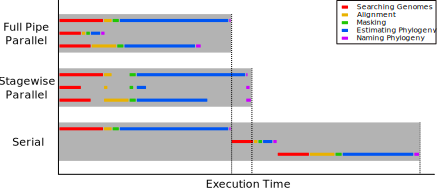
\includegraphics[width=\textwidth]{dendrogenous_parallel.pdf}
    \caption{A explanatory plot showing 3 different possible architectures for a tree generation pipeline. 
        Serial, in which each phylogeny is run one after another.  This form makes no use of multiprocessing
        facilities, however, a moderate but significant performance improvement can be achieved by allowing
        each stage in the pipeline to utilise multiple cores i.e. the trees are generated serially but during
        their generation alignment and blasting making use of multiple processors.          
        Stagewise parallel, where for example, all alignments for each input sequence are run side-by-side 
        and masking begins once the last sequence has finished alignment.  The disadvantage of this is a single
        slow stage for one input sequence can hold up the whole pipeline and leave resources idle.  Additionally,
        by running many of the same type of process at the same time, each with similar resource requirements,
        the risk of hardware bottlenecking is increased compared to a more heterogenous load.
        Finally, fully parallel runs each input sequence through the pipeline stage-by-stage separately
    from all other inputs to the pipeline. This prevents blocking and allows efficient using of resources.}
    \label{fig:ddg}
\end{figure}

40 genomes covering the diversity of the tree of life, with a particular focus on green algal and ciliate representatives 
were selected for this phylogenetic generation.
\textit{Arabidopsis thaliana}, \textit{Chlamydomonas reinhardtii},
\textit{Ostreococcus tauri}, \textit{Micromonas pusilla CCMP1545},  \textit{Chlorella variabilis NC64A}
\textit{Chlorella vulgaris C-169}, \textit{Physcomitrella patens}, \textit{Saccharomyces cerevisiae S288C}, 
\textit{Neurospora crassa OR74A},
\textit{Homo sapiens},
\textit{Mus musculus},
\textit{Dictyostelium discoideum},
\textit{Paramecium caudatum},
\textit{Paramecium tetraurelia},
\textit{Tetrahymena thermophila macronucleus},
\textit{Oxytricha trifallax},
\textit{Toxoplasma gondii},
\textit{Guillardia theta},
\textit{Bigelowiella natans},
\textit{Emiliania huxleyi CCMP1516},
\textit{Aureococcus anophagefferens},
\textit{Ectocarpus siliculosus},
\textit{Schizosaccharomyces pombe},
\textit{Bacillus cereus ATCC 14579},
\textit{Escherichia coli str. K-12 substr. MG1655},
\textit{Escherichia coli O157 H7 str. Sakai},
\textit{Salmonella enterica subsp. enterica serovar Typhi str. CT18},
\textit{Amycolatopsis mediterranei U32},
\textit{Aquifex aeolicus VF5},
\textit{Borrelia burgdorferi B31},
\textit{Chlamydophila pneumoniae CWL029},
\textit{Chlorobium tepidum TLS},
\textit{Deinococcus radiodurans R2},
\textit{Caulobacter crescentus CB15},
\textit{Sulfolobus islandicus M.14.25},
\textit{Nanoarchaeum equitans Kin4-M},
\textit{Haloferax mediterranei ATCC 33500},
\textit{Methanococcus maripaludis S2},
\textit{Cenarchaeum symbiosum A}.

\subsubsection{Automated Phylogenetic Transcript Binning - Arboretum}
In order to automate phylogeny based transcript binning the 10,000
manually verified phylogenetic bins from the initial BLAST based binning
and analysis were used as a training dataset for supervised classification.

The supervised classification was implemented in a script called ``Arboretum''
The cardinalities of each label in training set was relatively balanced (all within
the same order of magnitude) 1975 endosymbiont phylogenies, 2600 host, 3456 food, and 1969
unknown. 

``Arboretum'' parses phylogenies and identifies the k (default of 10) nearest branches to the seed transcript
the phylogeny was generated from.  The species of these closest leaves is queried taxonomically using the
NCBI taxonomy local database implemented in the ETE toolkit.  With a set of look-up filters e.g.
sequences from ciliates can be defined as "host-like", a set of vectors is created for each phylogeny.  
These are N-dimensional vectors where N is the number of class labels being used. 
For example, in this specific case: "endosymbiont", "host", "food/bacterial", and "unknown".
The magnitude of each dimension is the summed reciprocal phylogenetic distance between the root node and all
of the nearest branches that have been identified as being indicative of a certain class.

1,000 vectors from this training set were held out to form the test set and all models were then trained
using stratified 5-fold cross-validation on the remaining 9,000 training vectors. 
Support vector machines, random forest and logistic regression algorithms as implemented in scikit-learn 
were evaluated for performance manually and best performing classification algorithm was selected.
Additionally, an autoML method in which all available models are considered as hyperparameters in an efficient
bayesian optimisation approach was also attempted \citep{Komer2014}. 
Model performance was evaluated using a weighted average of all against one f1-scores as implemented 
in scikit-learn.

Input data was plotted using t-distributed stochastic neighbour embedding implemented in scikit-learn.

\section{Results} 

\subsection{Library contamination screening}

Libraries were screened for inclusion in assemblies by inspection of their taxonomic
profiles (see \ref{tab:sct_duey} and \ref{tab:bulk_duey}) as determined by DueyDrop 
and their GC\% probability densities (via KDE).

The GC density estimates of the single cell libraries show a clear bimodal GC density
with a high 70GC\% peak (\ref{fig:gc_prop_raw}) in all dark single cell libraries. 
With the exception of Dark1-2 and Dark2-3 this high GC peak is a greater density
than the expected peak 30-50GC\% (from known GC\% found in genomes
of sequenced relatives of both host and endosymbiont).

\begin{figure}[h]
    \includegraphics[width=\textwidth]{lib_gc_prop.svg}
    \caption{Probability densities of per-read GC proportions for the raw data (apart from pretrimmed bulk explained previously)
        from each sequenced library 
        Densities were derived using Kernel Density Estimation implemented in Seaborn. 
        The bulk and single cell light libraries demonstrate similar shaped distributions
        although the bulk has a greater proportion of low GC\% reads potentially representing
        more \textit{Paramecium} derived data. All single cell dark libraries 
        demonstrate a bimodal density with up to the majority of reads deriving 
        from an unknown high 70\% GC population. The dark single cell libraries
        exhibiting a relatively larger peak at 70\% GC than at 40-50\%GC (i.e.
        Dark1-3, Dark1-5, Dark2-2, Dark2-7) were
        the same libraries which were identified as potentially contaminated
        in taxonomic screening (see \ref{tab;sct_duey}).
    }
    \label{fig:gc_prop_raw}
\end{figure}

When these KDE are compared to the densities estimated from the Q20 trimmed
bulk reads (bottom right pane in \ref{fig:gc_prop_raw}) and 
raw bulk RNAseq reads from \citep{Kodama2014} (see \ref{fig:gc_prop_kodama}) 
it is apparent that this high GC\% peak is likely originating from
a high GC\% bacterial contaminant in the Dark single cell libraries.  

One other observation when comparing the bulk RNAseq analyses to the single cell
libraries is that the main GC peak is slightly lower in the bulk (and Kodama dataset), 
around 30GC\% versus 45-50GC\%.
This possibly indicates a greater proportion of reads deriving from the low
GC\% \textit{Paramecium bursaria} host and fewer from the 50GC\% endosymbiont
in bulk libraries relative to single cell libraries.  

\begin{figure}[h]
    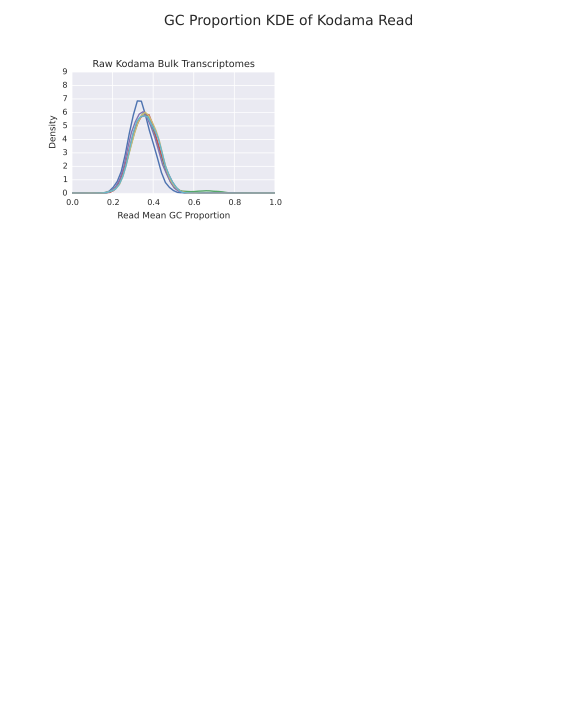
\includegraphics[width=\textwidth]{kodama_gc_prop.svg}
    \caption{Probability density of the per-read GC proportion for raw data derived from
    \citep{Kodama2014} transcriptome analysis of a different \textit{P. bursaria} species
with and without its endosymbiont. This dataset displays densities relatively similar
to the bulk RNAseq conducted in this project - "Trimmed Bulk Libraries in \ref{fig:gc_prop_raw}}
    \label{fig:gc_prop_kodama}
\end{figure}

By comparing the results of the KDE GC analysis with and without read trimming it
is apparent that trimming of reads makes nearly no difference in the density estimates.
The KDE of Q30 sliding window trimmed single cell reads in \ref{gc_prop_q30} is nearly
identical to that of the raw reads \ref{fig:gc_prop_raw}.

\begin{figure}[h]
    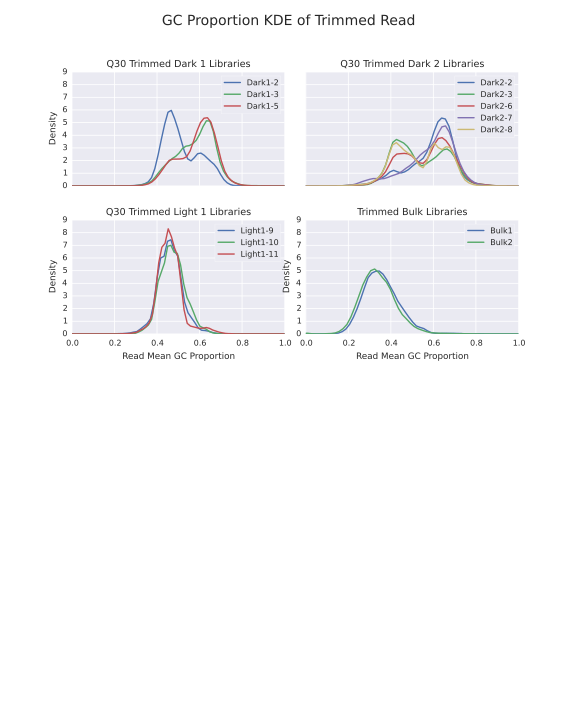
\includegraphics[width=\textwidth]{lib_gc_prop_q30_trimmed.svg}
    \caption{Probability densities of per-read GC proportions for trimmed reads.
             To ensure probability densities estimated in \ref{fig;gc_prop_raw}
         weren't biased by low quality ambiguous reads the same analysis was
     repeated using reads trimmed using a sliding window approach with a stringent average
 quality threshold of Q30.  In all cases the densities produced appear near identical to
 the analysis of the raw data}
    \label{fig:gc_prop_q30}
\end{figure}

The taxonomic profiles of single cell (\ref{tab:sct_duey}) and bulk libraries (\ref{tab:sct_bulk}) 
generated by DueyDrop are summarised in the tables below.  It is readily apparent 
that Dark1-3, Dark1-5, Dark2-2, and Dark2-7 display an aberrantly low number of reads
aligning to known alveolate (or even eukaryote) sequences. 
Forward and reverse reads within a library display similar profiles with a slightly
lower proportion of hits in the reverse reads. This can likely be attributed to
the lower read quality found in reverse reads relative to forward reads 
in paired-end Illumina sequencing. 

\begin{table}[h]
     \begin{tabular}{|l|l|l|l|l|l|l|l|}
         \cmidrule(r){1-6} \cmidrule(l){8-8}
         \textbf{SCT Library} & \textit{\textbf{Paired End Read}}          & \textbf{Eukaryote} & \textbf{Bacteria} & \textbf{Alveolate} & \textbf{Viridiplantae} &  & \textbf{Total Hits} \\ \cmidrule(r){1-6} \cmidrule(l){8-8} 
         \textit{Light1-9}    & \textit{R1}                   & 51.89 +/- 0.45     & 9.37 +/- 0.26     & 25.15 +/-  0.71    & 7.45 +/- 0.33          &  & 69.49 +/- 0.37      \\ \cmidrule(lr){2-2}
                              & \textit{R2}                   & 51.75 +/- 0.25     & 8.82 +/- 0.24     & 24.85 +/- 0.56     & 7.49 +/- 0.21          &  & 68.75 +/- 0.29      \\ \cmidrule(r){1-6} \cmidrule(l){8-8} 
         \textit{Light1-10}   & \textit{R1}                   & 46.35 +/- 0.56     & 15.72 +/- 0.46    & 22.96 +/- 0.24     & 6.94 +/- 0.26          &  & 68.73 +/- 0.30      \\ \cmidrule(lr){2-2}
                              & \textit{R2}                   & 46.12 +/- 0.83     & 15.14 +/- 0.48    & 23.13 +/- 0.38     & 6.99 +/- 0.37          &  & 68.73 +/- 0.30      \\ \cmidrule(r){1-6} \cmidrule(l){8-8} 
         \textit{Light1-11}   & \textit{R1}                   & 58.28 +/- 0.47     & 3.62 +/- 0.12     & 28.68 +/- 0.43     & 8.20 +/- 0.40          &  & 71.38 +/- 0.49      \\ \cmidrule(lr){2-2}
                              & \textit{R2}                   & 57.74 +/- 0.27     & 3.50 +/- 0.10     & 28.23 +/- 0.36     & 8.41 +/- 0.31          &  & 70.42 +/- 0.20      \\ \cmidrule(r){1-6} \cmidrule(l){8-8} 
         \textit{Dark1-2}     & \textit{R1}                   & 28.64 +/- 0.51     & 22.88 +/- 0.61    & 12.23 +/- 0.28     & 4.93 +/- 0.19          &  & 60.31 +/- 0.49      \\ \cmidrule(lr){2-2}
                              & \textit{R2}                   & 28.29 +/- 0.24     & 21.06 +/- 0.21    & 12.13 +/- 0.28     & 4.87 +/- 0.34          &  & 57.65 +/- 0.35      \\ \cmidrule(r){1-6} \cmidrule(l){8-8} 
         \textbf{\textit{Dark1-3}}     & \textit{R1}          & 9.48 +/- 0.43      & 25.07 +/- 0.42    & 2.15 +/- 0.13      & 2.60 +/- 0.27          &  & 41.43 +/- 0.68      \\ \cmidrule(lr){2-2}
                              & \textit{R2}                   & 8.89 +/- 0.19      & 23.11 +/- 0.52    & 2.13 +/- 0.16      & 2.45 +/- 0.18          &  & 38.50 +/- 0.46      \\ \cmidrule(r){1-6} \cmidrule(l){8-8} 
         \textbf{\textit{Dark1-5}}     & \textit{R1}          & 5.56 +/- 0.19      & 23.99 +/- 0.44    & 1.07 +/- 0.07      & 2.89 +/- 0.11          &  & 36.72 +/- 0.33      \\ \cmidrule(lr){2-2}
                              & \textit{R2}                   & 4.94 +/- 0.21      & 21.75 +/- 0.53    & 1.02 +/- 0.11      & 2.33 +/- 0.17          &  & 33.06 +/- 0.52      \\ \cmidrule(r){1-6} \cmidrule(l){8-8} 
         \textbf{\textit{Dark2-2}}     & \textit{R1}          & 12.32 +/- 0.25     & 9.81 +/- 0.19     & 3.73 +/- 0.16      & 4.33 +/- 0.17          &  & 27.65 +/- 0.47      \\ \cmidrule(lr){2-2}
                              & \textit{R2}                   & 11.53 +/- 0.15     & 9.00 +/- 0.17     & 3.67 +/- 0.22      & 3.74 +/- 0.12          &  & 25.71 +/- 0.39      \\ \cmidrule(r){1-6} \cmidrule(l){8-8} 
         \textit{Dark2-3}     & \textit{R1}                   & 32.07 +/- 0.31     & 7.43 +/- 0.15     & 12.81 +/- 0.21     & 4.71 +/- 0.21          &  & 48.42 +/- 0.53      \\ \cmidrule(lr){2-2}
                              & \textit{R2}                   & 32.47 +/- 0.24     & 6.68 +/- 0.21     & 13.11 +/- 0.43     & 4.58 +/- 0.12          &  & 47.92 +/- 0.28      \\ \cmidrule(r){1-6} \cmidrule(l){8-8} 
         \textit{Dark2-6}     & \textit{R1}                   & 24.11 +/- 0.28     & 8.55 +/- 0.11     & 9.04 +/- 0.35      & 5.27 +/- 0.15          &  & 41.69 +/- 0.45      \\ \cmidrule(lr){2-2}
                              & \textit{R2}                   & 22.89 +/- 0.55     & 7.44 +/- 0.17     & 8.74 +/- 0.49      & 4.36 +/- 0.24          &  & 38.85 +/- 0.58      \\ \cmidrule(r){1-6} \cmidrule(l){8-8} 
         \textbf{\textit{Dark2-7}}     & \textit{R1}          & 9.96 +/- 0.24      & 16.89 +/- 0.27    & 4.22 +/- 0.24      & 2.83 +/- 0.17          &  & 37.06 +/- 0.40      \\ \cmidrule(lr){2-2}
                              & \textit{R2}                   & 8.77 +/- 0.18      & 15.00 +/- 0.43    & 3.94 +/- 0.14      & 2.16 +/- 0.11          &  & 32.86 +/- 0.29      \\ \cmidrule(r){1-6} \cmidrule(l){8-8} 
         \textit{Dark2-8}     & \textit{R1}                   & 28.24 +/- 0.48     & 4.45 +/- 0.13     & 12.00 +/- 0.32     & 4.69 +/- 0.06          &  & 40.50 +/- 0.37      \\ \cmidrule(lr){2-2}
                              & \textit{R2}                   & 28.22 +/- 0.47     & 4.30 +/- 0.22     & 11.98 +/- 0.37     & 4.32 +/- 0.24          &  & 40.05 +/- 0.22      \\ \cmidrule(r){1-6} \cmidrule(l){8-8} 
     \end{tabular}
     \caption{Taxonomic profiles of raw single cell libraries generated using ``DueyDrop''. All values are percentage of reads mapping to that category +/- the standard deviation between sample replicates.  Libraries
     highlighted in bold were those excluded from subsequent analysis on the basis of their very low numbers of reads identifiable as 
 eukaryote (or specifically alveolate or archaeplastida). All forward and reverse read pairs display similar profiles to one another suggesting
 the problem of ``MDA chimeras'' may be minor.}
 \label{tab:sct_duey}
\end{table}

The bulk libraries demonstrate a very low level of hits compared to single cell libraries (see \ref{tab:bulk_duey}), 
to the point where if they were single cell libraries they would be taxonomically excluded. 
However, it should be noted that the bulk libraries were sequenced on a Gene Analyzer II and are on average
half the length of single cell reads (76bp vs 150bp). Due to the difficulty aligning short reads
to references the difference between libraries may be attributable to this alone. 
Additionally, the vast majority of the lower number of hits do align to eukaryote (and alveolate) 
taxa consistent with an non-contaminated library. 

\begin{table}[h]
     \begin{tabular}{@{}|l|l|l|l|l|l|l|l|@{}}
         \cmidrule(r){1-6} \cmidrule(l){8-8}
         \textbf{Bulk Library} & \textit{\textbf{PE}} & \textbf{Eukaryote} & \textbf{Bacteria} & \textbf{Alveolate} & \textbf{Viridiplantae} &  & \textbf{Total Hits} \\ \cmidrule(r){1-6} \cmidrule(l){8-8} 
         \textit{Light}    & \textit{R1}              &  9.66 +/- 1.55     & 0.18 +/- 0.13     &  6.28 +/- 1.41     &  0.86 +/- 0.3          &  &  10.10 +/- 1.48       \\ \cmidrule(lr){2-2}
                              & \textit{R2}           &  9.62 +/- 0.81     & 0.26 +/- 0.09    &  6.58 +/- 0.36     &  1.04 +/- 0.41         &  &  10.16 +/- 0.95      \\ \cmidrule(r){1-6} \cmidrule(l){8-8} 
         \textit{Dark}   & \textit{R1}                &  4.90 +/- 0.78     & 0.36 +/- 0.11    &  3.14 +/- 0.58     &  0.50 +/- 0.16        &  &  5.40 +/- 0.93      \\ \cmidrule(lr){2-2}
                              & \textit{R2}           &  5.50 +/- 1.25     & 0.22 +/- 0.19   &  3.82 +/- 0.81     &  0.50 +/- 0.12         &  &  6.02 +/- 1.22      \\ \cmidrule(r){1-6} \cmidrule(l){8-8} 
    \end{tabular}
    \caption{Taxonomic profile of the bulk transcriptome samples generated using ``DueyDrop''.}
    \label{tab:bulk_duey}
\end{table}

To attempt to identify the likely source of the high GC\% contamination 
and to assess how representative the taxonomic profiling of small random
subsamples of reads \(\leq1\%\) to full scale analyses Krona was used to 
create interactive hierarchial plots of the taxonomic profiles. 
From this, Rhizobia species are the most prevalent high GC\% species found in the libraries
with this high 70GC\% peak in the KDE plots and therefore are the most likely source
of this particular aspect of contamination. 

\begin{figure}[h]
    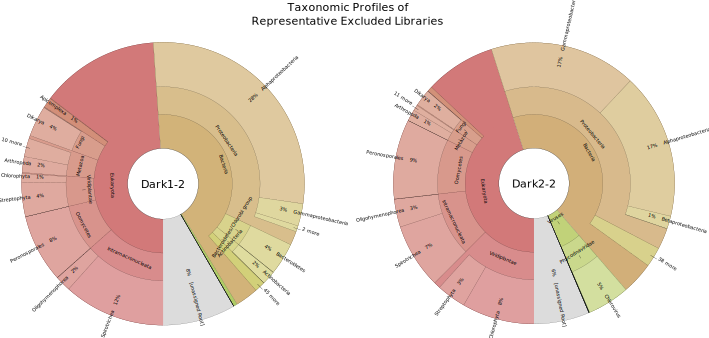
\includegraphics[width=\textwidth]{krona_excluded_raw.pdf}
    \caption{Krona visualisation of taxonomic profiles of representative
    single cell libraries that were excluded from further analysis due 
    to aberrant profiles (typically large proportion of reads being assigned
    to Bacteria than Eukaryota).  
    \label{fig:krona_excluded}
\end{figure}

\begin{figure}[h]
    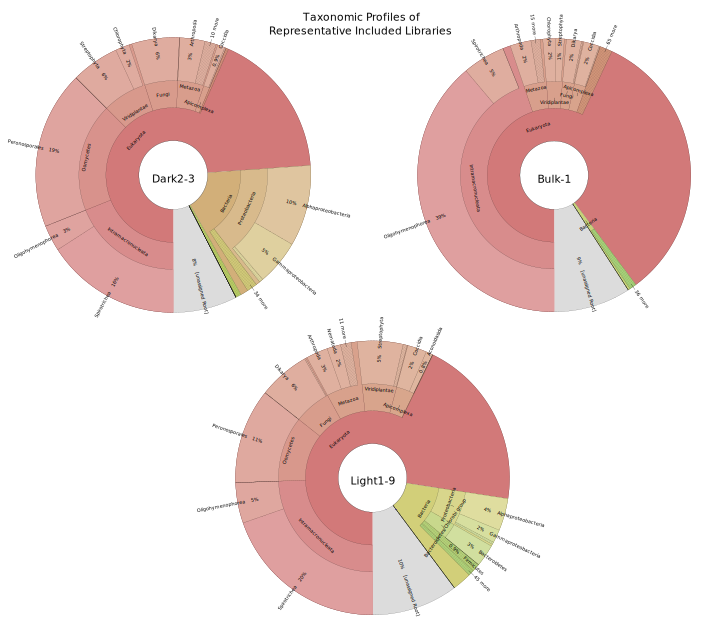
\includegraphics[width=\textwidth]{krona_included_raw.pdf}
    \caption{
    Krona visualisation of taxonomic profiles of representative
    single cell libraries that were excluded from further analysis due 
    to aberrant profiles (typically large proportion of reads being assigned
    to Bacteria than Eukaryota).  
    }
    \label{fig:krona_included}
\end{figure}


\begin{figure}[h]
    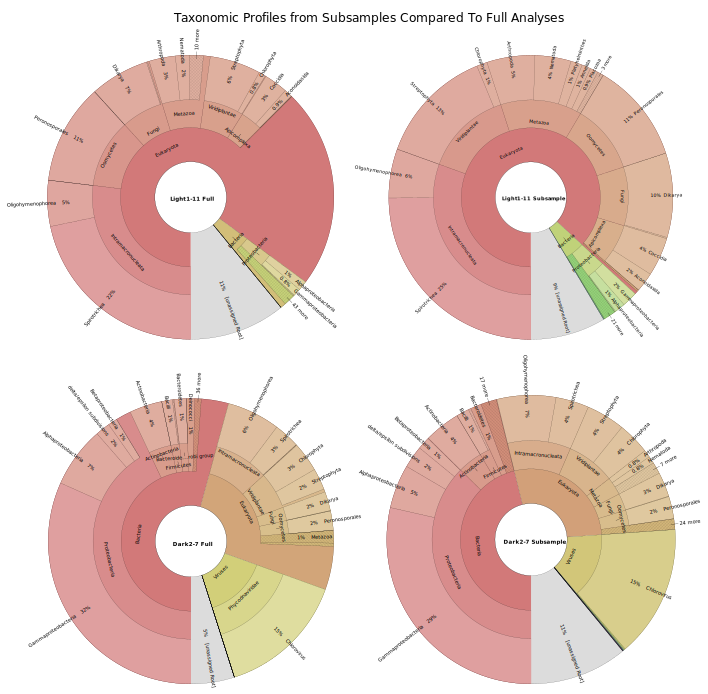
\includegraphics[width=\textwidth]{krona_all_vs_sample.pdf}
    \caption{Comparison of taxonomic profiles derived from small \(\leq1\%\)
        random subsamples of libraries compared to profiles generated using the
        full library.  Light1-11 and Dark2-5 are used as representative examples
        as they display the trends common for all single cell libraries. 
        All subsamples demonstrated taxonomic profiles with relatively similar
        proportions to full analyses.  For example, in the Light1-11 subsample
        of reads with hits the proportion of eukaryote to Bacteria was 87:4 
        \% vs 85:4\% of the root for the full analysis. Similarly the ratios
        for Dark2-7 shown eukaryote to bacteria are 26:54 for full analysis
        and 28:46 for subsample. 
        The key difference is the assignment of a greater proportion of reads to 
        intermediate taxonomic levels in the full analyses due to the difference in 
        resolution of multiple hits per read.  Principally, the full library analyses
        retain all hits and assign level based on a lowest common ancestor algorithm
        whereas the subsample analysis just uses the top hit.
    }
    \label{fig:krona_sample_vs_full}
\end{figure}


\subsection{Assembly Preprocessing} 

\subsubsection{Trimming Optimisation}

The optimal trimming threshold was determined by a combination
of read mapping statistics against 3 preliminary reference assemblies
as well as the impact on resultant \textit{de novo} assemblies at 
that threshold.

A rapid decrease in the number of concordantly mapping PE reads (i.e.
within insert distance of one another) was observed above a Q30 quality threshold.
This proves true regardless of the reference assembly being mapped to
(see \ref{fig:trimmingopt}).  Q30 relative to Q20 appears to induce a 
slight decrease in total number of mapping reads but not drastically slow 

\begin{figure}
    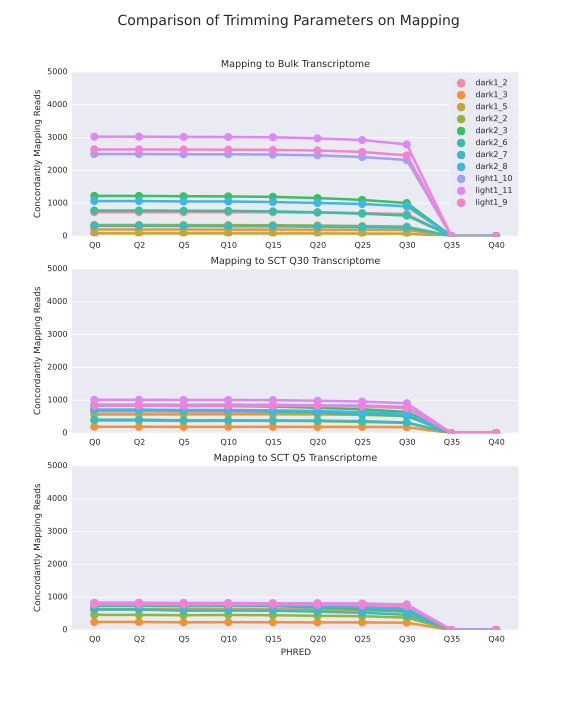
\includegraphics[width=\textwidth]{trimmingopt.svg}
    \caption{Assessment of the optimal minimum average quality threshold
             in Trimmomatic's sliding window (size 4) trim.  Plots
             display the number of concordantly mapping reads (forward
                 and reverse read map to assembly within their insert
             distance of one another) at a range of different trimming
             thresholds.  5000 randomly sampled PE reads 
             from each single cell library are mapped against 3 different 
             reference assemblies. 
             The key finding is above a threshold of Q30 there is a huge
         decrease in the number of mapping reads.}
         \label{fig:trimmingopt}
\end{figure}

Additionally, naive assemblies in Trinity of taxonomically screened single cell libraries
at different sliding window quality threshold trims of Q5, Q20, and Q30 (\ref{tab:trim_assembly})
were created. 
These show that more permissive trims (Q5 and Q20) lead to a greater number of assembled bases and transcripts 
however the likelihood of these assemblies are also lower than that generated using the 
more conservative Q30 trim. 
However, it should be noted that the difference in the number and size of assembled transcripts at different thresholds 
was less than was found using different assemblers and assembly parameters.

\begin{table}[h]
     \begin{tabular}{@{}|l||l|l|l|@{}}
         \cmidrule(r){1-6} \cmidrule(l){8-8}
         \textbf{Trim Threshold} & \textbf{Number of Transcripts} & \textbf{Bases Assembled} & \textbf{RSEM Assembly Likelihood} \\
         \cmidrule{}
         Q5 &  112,182 & 52,511,552 & \(-3.168*10^{10}\) \\
         Q20 & 107,955 & 50,809,686 & \(-3.015*10^{10}\) \\
         Q30 & 99,784 & 47,313,963 &  \(-2.832*10^{10}\) \\ 
    \end{tabular}
    \caption{Comparison of Trinity assemblies of taxonomically screened
        single cells reads (no bulk reads) at 3 different sliding window
        minimum average quality trimming thresholds.  Trimming largely
        does not cause a major difference between assemblies in terms of number
        of contigs recovered or overall likelihood with harsher trims resulting
        is slightly smaller but slightly more likely assemblies.
    }
    \label{tab:trim_assembly}
\end{table}

Therefore, due to increasing the assembly likelihood while only very marginally
marginally decreasing the number of contigs and mapping reads relative to
more permissive trims Q30 was determined to be the optimal trimming threshold.
It can be considered from this data that Q30 forms a maximum feasible stringency for trimming. 

\begin{table}
    \begin{tabular}
        \textbf{Library} & \textbf{Number of raw PE Reads} & \textbf{Number of Q30 trimmed PE Reads} \\
        \cmidrule{}
        Dark1-2 &  \(6.460*10^{7}\) &  \(3.355*10^{6}\)\\ 
        Dark2-3 & \(2.243*10^7\)&  \(1.478*10^7\)\\
        Dark2-6 & \(2.431*10^7\) & \(1.443*10^7\) \\
        Dark2-8 & \(2.761*10^7\) &  \(1.866*10^7\) \\
        Light1-9 & \(1.524*10^7\) & \(1.382*10^7\) \\
        Light1-10 & \(1.614*10^7\) & \(1.478*10^7\) \\
        Light1-11 & \(1.474*10^7\) & \(1.334*10^7\) \\
        Bulk1 & - & \(2.458*10^{7}\) \\
        Bulk2 & - & \(2.779*10^{7}\) \\
    \end{tabular}
\end{table}

\subsubsection{GC Partitioning} 

GC partitioning was conducted on Q30 trimmed reads 
using K-means clustering as implemented in the parKour tool described above 
to attempt to remove GC\% rich contamination from single cell libraries.

The 2 different clustering schemes attempted using 2 and 3 target clusters.
Additionally, both clustering schemes were also run with an initial overclustering factor of 3
i.e. parKour originally found 6 and 12 clusters and then merged them to produce the target 2 and 3 
clusters respectively. 

\begin{table}
    \begin{tabular}{ccr}
        \toprule
        Clustering Scheme & Centroids & Number of Reads Assigned \\
        \midrule
        \midrule
        2                    & (0.6674, 0.6177) & 57.3M \\
                             & (0.4557, 0.4393) & 81.6M \\
        \midrule
        2 (overclustering)   & (0.6672, 0.6168) & 57.7M \\
                             & (0.4555, 0.4392) & 81.2M \\
        \midrule
        3                    & (0.5363, 0.5092) & 44.0M \\
                             & (0.6924, 0.6394) & 43.3M \\
                             & (0.4231, 0.4096) & 51.6M \\
        \midrule
        3 (overclustering)   & (0.5365, 0.5090) & 43.9M \\
                             & (0.6921, 0.6396) & 43.6M \\
                             & (0.4235, 0.4098) & 51.7M \\
        \bottomrule
    \end{tabular} 
    \caption{Final cluster centroids and number of reads assigned
    to each cluster in parKour using various run settings.  Overclustering
made a minimal impact on cluster location}
    \label{tab:centroids} 
\end{table} 

2 and 3 target clusters with and without an initial 
overclustering factor of 3 (i.e. initially finding 6 and 12 clusters originally before merging to
produce final 2 and 3 cluster targets). 

Therefore, as can be seen overclustering made a minimal effect on cluster centroids and read assignment.

\begin{figure}
    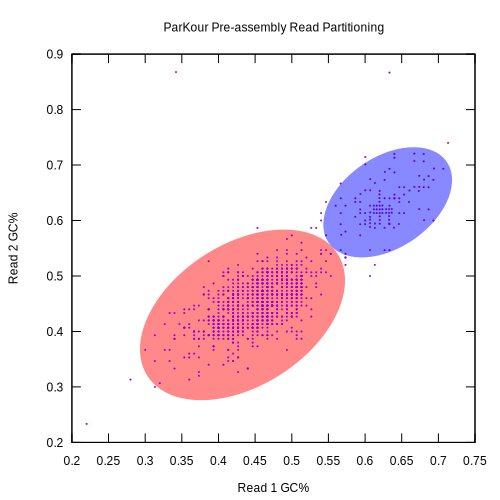
\includegraphics[width=\textwidth]{parKour.pdf}
    \caption{Visualisation of GC-based paired read K-means clustering on a small random subset of all single cell transcriptome
    reads. 2 initial centroids were specified without an overclustering factor and approximate final centroids (0.6674, 06177) and (0.4557, 0.4393) are indicated by highlighted areas.  57.3M and 81.7M were assigned to each respective cluster. Comparison to other clustering regimes can be found in \ref{tab:centroids}} 
        \label{fig:parkour} 
\end{figure}

Unfortunately, as might have been forseen, the resultant assemblies from individual
read clusters displayed high levels of fragmentation regardless of the clustering
regime used.  For example, in the case of the 2 cluster (without overclustering) 
and subsequent individual Trinity-based assemblies resulted in 268,806 transcripts
of marginally shorter average length than the equivalent unprepartioned assembly
(99,784 transcripts).

The same pattern, consistent with assembly fragmentation, 
was observed when only dark single cell libraries were clustered using 
2 or 3 clusters. 
Therefore, GC-based pre-assembly read partitioning proved incapable of improving
the assembly of this highly heterogeneous RNAseq dataset.


\subsubsection{Error Correction}

Bayeshammer, as implemented in the Spades genome assembler, even on permissively trimmed
(\(Q>5\)) reads corrected only a maximum \(0.0007\%\) of reads in the 7 taxonomically selected SCT libraries.
As this affected on the order of 10s of reads it was not considered worth pursuing further.

``SEECER'', an RNA-Seq specific error correction tool corrected 
``SEECER'' was used to correct lightly trimmed (Q5) SCT reads.  
Approximately, \(0.5\%\) of reads per library were corrected.

Trinity assemblies of just taxonomically selected single cell libraries were
then compared with and without ``SEECER'' error correction.
\begin{table}[h]
     \begin{tabular}{@{}|l||l|l|l|@{}}
         \cmidrule(r){1-6} \cmidrule(l){8-8}
         \textbf{Trim Threshold} & \textbf{Number of Transcripts} & \textbf{Bases Assembled} & \textbf{RSEM Assembly Likelihood} \\
         \cmidrule{}
         Q5 &  112,182 & 52,511,552 & \(-3.168 * 10^{10}\) \\
         Q5 SEECER Corrected & 111,853 &  51,847,128 & \(-3.147*10^{10}\) \\
         Q30 & 99,784 & 47,313,963 & \(-2.912*10^{10}\)  \\ 
    \end{tabular}
    \caption{Naive Trinity assembly of Q5 trimmed taxonomically selected single cell libraries
        with and without SEECER error correction.}
    \label{tab:trim_assembly}
\end{table}

As can be observed, error correction of SCT reads made minimal effect in the overall likelihood
or assembly for this dataset even with lightly trimmed reads. As this marginally
performed worse than the more stringent Q30 trim error correction was considered
ineffective on this dataset and was not used for further analysis.

\subsubsection{Digital Normalisation} 

Digital normalisation and removal of likely erroneous k-mers (i.e. low abundance) 
reduced the total input reads from the Q30 trimmed taxonomically
filtered SCT and bulk libraries from 
\(2.912*10^{8}\) to \(8.473*10^6\) paired reads.

Of those, \(6,231*10^{6}\) derive from the bulk and \(2.253*10^6\) 
from single cell libraries. 
Therefore, as Q30 trimmed single cell libraries comprised
\(9.318*10^{6}\) paired end reads and bulk libraries 
consisted of \(52.377*10^6\) reads digital normalisation
and abundance filtering resulted in a retention of 
\(2.418\%\) of single cell PE reads and \(11.891\%\) of
bulk PE reads.

This had a very positive effect on assembly in Trinity improving the assembly likelihood
by an order of magnitude while assembly more transcripts of near equal length (based on
median contig length).  In fact, the khmer processed assembly marginally increased
median contig length at the expense of a lower N50. 

%%%%%%%%%%%%<++> NOTE THIS IS Q30 with KHMER PROCESSING BUT NOT MINKMERCOV2 in TRINITY
\begin{table}[h]
     \begin{tabular}{@{}|l||l|l|l|l|l|@{}}
         \cmidrule(r){1-6} \cmidrule(l){8-8}
         \textbf{Preprocessing} & \textbf{Number of Transcripts} & \textbf{Bases Assembled} & \textbf{Contig N50} & \textbf{Median Contig Size} & \textbf{RSEM Assembly Likelihood} \\
         \cmidrule{}
         Q30 and Bulk &  127,508 & 83,264,944 & 851 & 411 & \(-2.832 * 10^{10}\) \\
         Q30 and Bulk with Khmer processing & 176,097 &  111,367,366  & 777 & 427 & \(-1.214*10^{9}\) \\  
    \end{tabular}
    \caption{Trinity assemblies of taxonomically selected single cell libraries
        and bulk libraries with and without digital normalisation and k-mer
        abundance filtering
    }
    \label{tab:diginorm_assembly}
\end{table}

As this both significantly improved assembly run time as well as the overall
assembly quality in Trinity digitally normalised and K-mer abundance filtered 
bulk and taxonomically selected Q30 trimmed single cell libraries were determined
to be the optimal pre-processing.

\subsection{Assembly}

\subsubsection{Referenced}

Referenced assembly using the divergent \textit{Chlorella NC64A},
\textit{Coccomyxa subellipsoidea} C-169, \textit{Tetrahymena thermophila},
\textit{Paramecium caudatum} genomes as references was largely ineffectual.
Of all bulk and SCT reads only 0.3 and 0.4\% mapped to the 
algal references.  Similarly, only 0.6 and 0.9\% of reads mapped to the 
respective ciliate genomes.   This level of mapping is on the order
of random chance.  The high proportion of reads which mapped, mapped non-uniquely
suggesting mapping was occurring in low complexity reasons and is a statistical
artefact for the most part instead of biological significant.

The addition of gene junction annotation files for the reference genomes to improve
spliced mapping only improved the percentage of reads mapping by 0.05-0.3 percentage points.  
With so few reads mapping, any attempt to 
class transcripts from this using cufflinks resulted in 10s of transcripts.

Therefore, referenced assembly using divergent related genomes proved impossible
for this dataset.

\subsubsection{\textit{de novo} assembly} 

\begin{table}[h]
    \begin{tabular}{|l|r r r r r r l}
        \textbf{Assembler} & \textbf{Parameters} & \textbf{Number of Contigs} & \textbf{Total Bases Assembled} & \textbf{Assembly Likelihood}\\
        SOAPdenovo-Trans & K23 & 374,325 & \(7.64*10^{7}\) & \(3.778*10^{10}\) \\
                         & *K64 & - & - & - \\  
                         & *K80 & - & - & - \\ 
        TransAbyss & K20 & 3,272,137 & \(1.722*10^{8}\)   & -  \\
                   & K32 & 853,079   & \( 1.321*10^{8}\)  & -  \\
                   & K64 & 376,280   & \( 9.755*10^{7}\)  & -  \\
                   & Merged & 3,055,851 & \(2.71*10^{8}\) & \(-3.113*10^{10}\)  \\
        Oases*     & - & - & - & - \\
        IDBA-tran      & - & 54,113 & \(2.7*10^{7}\) & \(-4.589*10^{10}\)\\
        IDBA-MTP/UD/MT** & - & - & - & \\
        Trinity & Minimum K-mer Coverage 2 & 127,508 &  \( 8.326*10^{7}\) & \(-2.832*10^{10}\) \\
        Bridger & K25 & 114,582 & \( 9.707*10^{7}\)  & \(-2.587*10^{10}\)\\ 
    \end{tabular}
    \caption{\textit{De novo} assemblies of Q30 trimmed taxonomically
        selected single cell libraries and bulk libraries (but not digitally normalised or k-mer abundance
            filtered) with a range of assemblers and parameters.  K-mer size used
            for assemblers with that option are indicated in the Parameters column 
            e.g. K23 indicates a 23-mers. Bridger and Trinity outperformed 
            other assemblers in terms of assembly likelihood and rational
            contig numbers and sizes.
        * indicates assemblies programs that failed to run to completion due to 
        insufficient computational resources (despite using a server with 500GB 
        of memory)
        ** indicates assemblies which failed due to coding errors in the application.
        All non-diginormed sct+bulk}
        \label{tab:assemblies}
\end{table}

Critically, Oases, the IDA-MTP/UD/MT pipeline and SOAPdenovo-Trans at higher K-mer values
all failed to run to completion correctly with the dataset.  In the case of Oases
and SOAPdenovo-Trans at higher K-mer values this was due to exhaustion
of system memory and in the case of IDBA-MTP/UD/MT workflow an unresolved coding error 
resulting in repeated segmentation faults.

However, Trinity and Bridger both consistently generated assemblies of approximately
equal size (100-130,000 contigs of rational sizes: N50s of 700-850
    and mean and median contig sizes of 600-660 and 410-470) across a variety 
    of assembly parameters (not shown).  Furthermore, they both consistently
    generated the assemblies with the greatest likelihoods (from RSEM-Eval), 
    and ran most computationally efficiently. 


Trinity and Bridger assemblies using digitally normalised and K-mer abundance 
filtered, taxonomically selected, Q30 trimmed, single cell and bulk libraries performed 
even better in terms of assembly likelihood and read incorporation.

\begin{table}[h]
    \begin{tabular}{|l|r r r r}
        \textbf{Assembler} & \textbf{Parameters} & \textbf{Contigs} & \textbf{Bases Assembled} & \textbf{Assembly Likelihood} \\
        Bridger & K19 & 102,686 & \(8,209*10^{7}\)  & \(-1.729*10^{9}\) \\
                & K25 & 113,106 & \(9.866*10^{7}\)  & \(-1.183*10^{9} \) \\ 
                & K31 & 112,391 & \(8.941*10^{7}\)  & \(-1.143*10^9\) \\ 
        Trinity & Minimum K-mer Coverage of 1 & 176,097 &  \(1.113*10^{8}\)& \(-1.214*10^{9}\) \\  
                & Minimum K-mer Coverage of 2 & 147,902 & \(9.239*10^{7}\) & \(-1.238*10^9\) \\  
    \end{tabular}
    \caption{Asssembly summaries of Q30 trimmmed taxonomically selected SCT and bulk reads 
    after digital normalisation and K-mer abundance filtering. Parameters used in the assembly
indicates any special parameter settings used in the assembly i.e. K19 indicates a K-mer size of 19 was used.
}
    \label{tab:digassemby}
\end{table}

Smaller K-mer values (19-mer) performed worse in the case of the Bridger assembly
with the optimal assembly in terms of contig number and size was the K-mer size 
of 25.  This was slightly lower in terms of likelihood than the 31-mer Bridger
assembly. The digitally normalised and filtered Trinity assemblies 
generated much larger assemblies overall but still produced good likelihoods.

\subsubsection{Assembly combination}

Two assemblies were combined using the tr2aacds.pl script in EvidentialGene 
and a minimum CDS size of 100. The first consisted of all successfully completed
assemblies of non-normalised/filtered reads i.e. SOAPdenovo-Trans, TransAbyss (multiple K-mer
assembly merged using built-in tool),
IDBA-tran, Trinity and Bridger in \ref{tab:assemblies}.  The second, 
of the 3 Bridger digitally normalised assemblies and two Trinity assemblies 
described in \ref{tab:digassemby}.

\begin{table}[h]
    \begin{tabular}
        \textbf{Assembly} & \textbf{Input Contigs} & \textbf{Collapsed Contigs} & \textbf{Assembly Likelihood}\\ 
        Non-normalised    & 3,726,379 & 46,063  & \(-4.347*10^{10}\) \\
        Normalised        & 652,182 & 53,628 & \(-1.823*10^{9}\)\\
    \end{tabular}
    \caption{Summary of merged multi-assemblies.  Collapsed contigs is the number of contigs
    found in the merged set by the EvidentialGene pipeline. The level of assembly
reduction and redundancy removal is very high and impressively consistent despite
the differences in the starting assemblies.  However, the likelihoods are lower than
any of the individual assemblies used in the combinations.}
    \label{tab:comb_assemb}
\end{table}

The combination of all non-normalised assemblies produced a suprisingly small
set of contigs, however, also both assemblies also had lower likelihoods than 
any of their constituent assemblies. It is of interest that despite both
generating similar numbers of contigs there was next to no overlap between 
the two combinations as assessed by clustering using CD-HIT at a similarity of \(90\%\).

Therefore, the assembly selected for downstream binning and analysis was Bridger 
assembly of bulk and library screened single cell normalised and k-mer
abundancy filtered reads with a K-mer size of 31.

\subsection{Binning}

\subsubsection{ORF Calling}

From the 112,391 contigs in the final selected assembly - 1,005,370 ORFs
longer than 30 amino acids were identified using a ``Tetrahymena'' encoding.
Using the 500 longest of these ORFs to train a Markov Model and removing
shorter ORFs that lay entirely within a longer ORF resulted in a final set
of 70,605 transcripts.

\subsubsection{Performance of BLAST binning alone}

10,000 of these transcripts were translated to peptide sequences 

The initial identification and binning of recovered transcripts into host and endosymbiont categories was 
tested using this phylogenetic approach. The results of this analysis is plotted 
below. This demonstrates that the initial bin identifications were accurate for
endosymbiont (~92\%) and food ( ~94\%) derived transcripts. 


\begin{figure}
    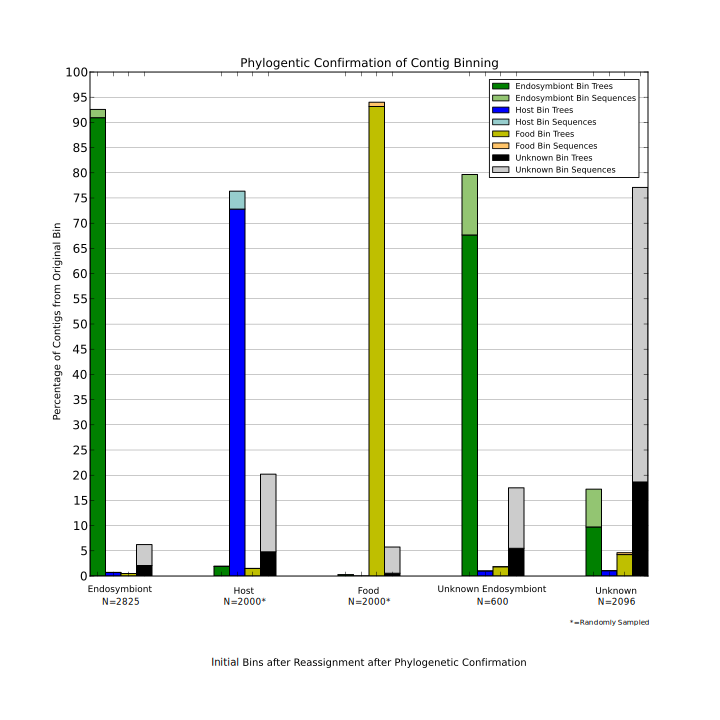
\includegraphics[width=\textwidth]{change_in_binning_after_phylogenetic_confirmation.pdf}
\end{figure}


\subsubsection{Phylogeny based bins}

\textbf{This needs recalculated}
%Of the bins that were too large to
%be comprehensively phylogenetically tested (‘Host Bin’ and ‘Food Bin’) we screened a subset
%of 2000 transcripts using a phylogenomic approach. There were almost no detected endosym-
%biont sequences in 2000 randomly selected ‘Food Bin’ transcripts therefore the ‘Host Bin’ was
%the only cause for concern in containing misidentified endosymbiont transcripts. ~2\% of the
%2000 randomly sampled ‘Host Bin’ transcripts were found to be wrongly identified endosym-
%biont sequences, assuming this random sample is representative of the ‘Host Bin’ in general
%this suggests 500 endosymbiont transcripts are misidentified as host sequences.


For automated classification, the random forest test score showed a 93\% accuracy and automl approach ensemble test scored at 87.3\% accuracy.
Dishearteningly, this is not massively more accurate than the crude BLAST based binning approach.
 

From these, 39,095 contigs 18,111 were generated using ``Dendrogenous''.  Unfortunately, nearly half had too few hits in the 40 genomes used 
to generate phylogenies.  \footnote{However, in speed testing ``Dendrogenous'' did prove very efficient at rapidly generating phylogenies with its
fully parallelised mode capable of generating 100 phylogenies randomly selected transcripts against 41 genomes in an average 2:22.50 minutes.
The same pipeline run serially took an average of 23:41.39 minutes and the stage-wise parallel was very marginally faster at 
an average of 21:45.02 minutes.}




\section{Discussion}

\subsection{Library screening is a key stage in sc-RNAseq}

Much as library contamination is one of the key issues with single cell genomics \citep{Blainey2013,Lusk2014}, it highly
important in SCT.  Single cell methods are particularly prone to contamination issues
from reagents, laboratory environment and enigmatic nucleic acids within the biological samples themselves.
This is due to the low-input concentration and high amplification necessary in these approaches \citep{Blainey2013} 
leading to enrichment of non-target sequences.

Furthermore, when utilising single cell libraries in a \textit{de novo} assembly instead of just referenced mapping assemblies
it is doubly important to discard libraries that are likely to be contaminated as they will severely complicate
the assembly graph. This increases both the hardware requirements to resolve transcripts from the de-Bruijn graph, as well
as reducing the accuracy of those recovered transcripts.  The importance of library screening was further emphasised
in the context of this projects by the observation that the inclusion of certain (SCT) libraries would increase
assembly run-time and lead to the generation of fragmented transcripts relative to assemblies without those
libraries.  While, contamination screening approaches such as multi-genome alignments and mapping to likely contamination
species have been developed (e.g. \citep{Hadfield2014}), they were largely insufficient as they tended to rely upon 
A) the contamination species being characterised and specified a-priori and B) the existence of reference genomes.
One interesting exception is that of the commercial \url{http://onecodex.com} platform which provides
rapid taxonomic screening of libraries as a cloud service.  While the emergence of commercial platforms
is additional evidence as to the utility of this form of screening, even onecodex is largely optimised
on common human pathogens.

Therefore, to this end a set of scripts, known as ``DueyDrop'', were developed to allow rapid taxonomic profiling of a
representative subset of each library against the entire non-redundant protein database.  
These profiles could then be manually analysed or grouped using unsupervised learning methods to investigate the existence of 
outlier libraries likely to be the product of contamination or sequencing failure.   Libraries can then,
based on the heuristics of the dataset, by discarded and retained for downstream assembly and analysis.

In order to discover whether trimming was necessary prior to screening, taxonomic profiles generated from raw untrimmed 
were compared to profiles from trimmed libraries. If trimming is not necessary prior to contamination screening
it saves a potentially computationally intensive step being run on libraries set for discarding.








Key, 

GC KDE can be informative in the case of contamination with GC diverse
species.

Trimming makes little difference.

Subsamples are representative of full samples.

Don't just take top hit, take all hits and use LCA.






Interestingly, these samples didn't appear to be uniformly especially enriched for likely bacteria derived reads or obvious contaminants
such as \citep{Homo sapiens}.  Therefore, it is unclear whether they represent lower quality 
libraries or a true sub-population of PbMr cells that has lower transcriptional activity.
Removal of these libraries halved the number of recovered transcripts in Trinity \textit{de novo} assemblies as can be seen in the the assembly
summaries below.



Despite evidence that nanoscale methods can greatly reduce levels of contamination \citep{Blainey2011}, the taxonomic profiling conducted here
indicates a high level of bacterial (and viral) contamination in the scRNA-Seq.  Intriguingly, similar taxonomic profiling of the bulk
libraries revealed a very low percentage of reads mapping to any sequence in the nr protein database.  This was significantly lower than the
sc-RNAseq libraries.  While this finding is concerning it is likely to be an artefact of the older sequencing platform the bulk data was generated on.
These paired reads were sequenced via the GAII and were half the length of the HiSeq2500 reads used for the SCTs.  Shorter reads and a relatively higher
technical error rate on this platform may have played a role in this marked decline in recognisable reads. 
Despite this the relative proportion of bacterial reads to eukaryote reads among the recognisable reads is much lower for bulk libraries than SCT.
This supports the findings of \citep{Kolisko2014}, in which enigmatic, bacterial contamination was a problem in single cell eukaryotic
transcriptomes.   One possible reason for this is that due to the high levels of amplification required, the poly-A selection step
in library prepartion is less effective at removing non-eukaryote mRNA transcripts.




Another, feature of the profiles of interest is the systematically low 
low levels of Viridiplantae related reads across both bulk and sc-RNAseq libraries and in both lit and dark conditions.  The most likely culprit for
this is inefficiencies in the lytic step of RNA extraction for \textit{Micractinium} cells. 
Lysis is difficult in cells
with cell walls \citep{Korfhage2015} and \textit{Micractinium} is known for its robust chitin walls. 

Finally, both SCT and bulk dark libraries reflect a significantly lower proportion of eukaryote mapping reads. Either dark expressed transcripts 
reflect a high degree of novel, previously unsequenced, diversity, other uncharacterised contaminants are active at night or there is some aspect
of the extracted material in the dark that leads to problematic sequencing.  

%One potential explanation for this last scenario could be 
%an aggravated AT bias leading to high sequencing error due to a relatively greater proportion of AT-rich host derived reads 

``DueyDrop'' could potentially be improved in such a way that an entire library can be screened instead of just subsamples.
Briefly, this would involve quantifying exact k-mer matches between library reads and a pre-generated database of known taxa
using efficient probabilstic hashing datastructures such as a bloom filter, or more likely count-min sketch and an efficient
k-mer counting library such as Jellyfish \citep{Marcais2011}.  This would have a major speed advantage compared to the BLASTX-based method of ``dueydrop''
and would thus allow entire libraries to be checked in reasonable time.  However, it would require laborious workarounds to handle
k-mers shared between multiple taxa in the database, translation of reads and/or database sequences into a matching sense and form (e.g. protein),
and use of a locality-sensitive hash function to handle scenarios where there is no exact k-mer match. This latter issue is particularly
problematic for libraries consisting of transcripts from poorly sampled reaches of the tree of life where exact matches would become
commensurately rarer as sampling sparsity increases.  
While still affected by this problem, the BLASTX/Diamond approach implemented in the ``DueyDrop'' scripts are relatively more robust to these
problems due the explicit probabilistic modelling of sequence divergence built into the BLAST alignment algorithm (e.g. E-values).

Regardless, taxonomic profiling and contamination screening had great utility identifying potential problems in library preparation (e.g. chitin lysis despite
additional bead disruption and freeze-thaw steps taken) as well as offer a powerful means of removing problematic libraries from assembly.






\subsection{Assembly optimisation}


Following contamination screening the next two key preprocessing steps are that of read trimming and error correction.
While there has been some analysis of the optimal trimming parameters for bulk RNAseq (particularly \citep{Macmanes2014})
there has not been an investigation of the optimal trimming parameters for single cell RNAseq Illumina reads.
Correct trimming is important to minimise sequence error (mostly substitutions \citep{Yang2013}) as these
result in assembly of spurious sequences \citep{Macmanes2013,Macmanes2014}.  Therefore, to determine
optimal trimming parameters for the raw single-cell paired-end RNA-Seq reads 
a naive grid search algorithm using random reads sub-sampled from each library was used and effect on mapping
statistics against a ``baseline'' Trinity assembly of bulk reads \citep{Haas2013}.

There has been emerging evidence that error correction is a key stage in the accurate
recapitulation of reads, especially from single cell libraries \citep{Medvedev2011}.  
Error-correction is typically achieved by discarding lowly expressed k-mers 
as these are likely to have been generated by errors.
Therefore, the effect and feasability 
of read error correction on assembly was also assessed using error correction algorithms developed specifically for either 
single cell (genomic) data or RNAseq data (but not necessarily sc-RNAseq data).
Digital normalisation, a method to remove redundant read data from libraries and thus
reduce the computational burden of assembly \citep{Brown2012}, was also investigated for this dataset.
Interestingly, some have argued that error correction is special case of general digital normalization
\citep{Krasileva2013}.


As we expect the PbMr metatranscriptome to contain predominantly a highly AT-rich organism, \textit{Paramecium},
(ranging from 24.1 to 28.2\%GC in \textit{P. aurelia} species complex and \textit{P. caudatum} \citep{Aury2006,McGrath2014})
and a very GC-rich organism, \textit{Micractinium}, (\textit{Chlorella variabilis} NC64A genome is approximately 67.1\%GC, the highest
found in a sequenced eukaryote genome (in 2010) \citep{Blanc2010}), the utility of pre-assembly read partioning was assessed.
This GC pattern was supported by the clear bimodal GC distribution that can be observed in \ref{fig:gc}.
Following a practice found in some meta-omic analyses (such as those in \citep{Droge2012}) in which reads
are partitioned and then the individual partitions are assembled separately a custom clustering
tool named ``parKour'' was created.  ``parKour'' uses unsupervised clustering of reads via K-Means 
and GC content.  Theoretically, accurate
pre-assembly read partitioning could transform a complex assembly graph into two relatively simpler
assembly tasks.  As well as simplifying path resolution accuracy, if this method were to work
it would speed up assembly considerably and thus allow more iterations to optimise other
assembly paramters.

\begin{figure}
    \includegraphics[width=\textwidth]{lib_gc_prop.pdf}
    \caption{Kernel Density Estimate \citep{Rosenblatt1956,Parzen1962} plots of the mean GC proportion per read within each single cell transcriptome library.
             Plots used a gaussian kernel and a bandwidth determined by ``Scott's normal reference rule'' \citep{Scott1979}.  Lines in each subplot represents a KDE
             of an individual sequencing library and they are displayed in subplots corresponding to their originating condition (``Light 1'', ``Dark 1'' 
             and ``Dark 2'') i.e. from the lit and dark libraries from the first sequencing run and the extra dark libraries generated in the second sequencing run.
             Shared colours between distinct subplots do not imply any common library identities. 
             The exception to this is the final plot which shows the GC proportion KDE of all single cell libraries combined.
             The bimodal probability distribution shown in all plots (and especially prevalent in the dark libraries and the combined KDE) is indicative 
             of the GC biases of \textit{P. bursaria} and \textit{M. reisseri} and the relative proportion of reads originating from these organisms in each library.
    \label{fig:gc}
\end{figure}

\subsubsection{Assembly and assembly assessment}

While an attempt can be made to identify optimal pre-processing
parameters using heuristic measures like mapping metrics against a reference. 
It is very difficult to identify the parameters (preprocessing or otherwise) which will leads to the ``best'' 
\textit{de novo} assembly prior to actually generating the assembly.
  Assembly can be considered an example of Wolpert and Macready's ``No Free Lunch Theorems'' \citep{Wolpert1995,Wolpert1997} 
  as (in the case of \textit{de novo} assembly) it is fundamentally a hamiltonian/eulerian cycle search problem (equivalent
    in the de-Bruijn formulation) and therefore any two assembly implementations (in different assemblers and/or
    with different parameters) should ultimately be equivalent across all possible input datasets.\footnote{
    This should be taken with a pinch of salt, a proof of this theorem applied to the case of assembly is beyond
both the scope of this thesis and my abilities}.  For this reason, it is necessary to try
assembly using a random of assembly parameters and indeed a range of both \textit{de novo} and referenced assemblers. 
For this reason, 4 \textit{de novo} assemblers were used: Trinity, SOAPdenovo, TransAbyss, and Velvet/Oases (see \ref{sec:methods} for details)
as well as Cufflinks/TopHat2/Bowtie2 for referenced assemblies.  However, as Trinity overwhelming generated the best 
\textit{de novo} assemblies in preliminary assemblies the majority of optimisation focussed on this assembler.


Unfortunately, the task of identifying the ``best'' \textit{de novo} transcriptome assembly is also a non-trivial 
task \citep{Neil2013}.  Many widely used assembly assessment metrics have been shown to be
inconsistent measures in simulated sequencing data, especially those metrics related to invidual
contigs (theoretically different transcript splices).  Metrics such as average length and N50
prove consistent across both simulated sequencing depth and read lengths i.e. they improve 
towards \citep{Neil2013}.  Furthermore, the number of possible metrics is greatly reduced
if assessment is mainly conducted in a reference-free manner \citep{Li2014}.  As the majority of
assemblies were \textit{de novo} and the suitability of the related but divergent genomes
as references was one area that was being investigated it was necessary to restrict to reference-free
assembly assessments.  Therefore, a model-based reference-free assembly scoring algorithm (RSEM-EVAL \citep{Li2014} was,
    along with standard (if imperfect) metrics, used to evaluate different assemblies. 







\subsubsection{Trimming}

There are many available tools for read-trimming (as discussed in \ref{ch:methods}),
and a range of trimming tools were initially
considered: specifically Trimmomatic \citep{Bolger2014a}, Sickle \citep{JoshiGitHub}, FASTX-toolkit \citep{gordon2010fastx},
PRINSEQ \citep{Schmieder2011} and cutadapt \citep{martin2011cutadapt}. 
Despite Sickle, an adaptive quality trimmer, having previously been used in single-cell transcriptome datasets 
from free-living eukaryotes \citep{Kolisko2014}, it proved suboptimal as it was
not capable of removing 5' or 3' contaminants such as sequencing adapters and/or multiplexing tags by itself.  
These stages could be achieved with individual tools (such as Skewer \citep{Jiang2014}, 
TagDust \citep{Lassmann2009} and Scythe \citep{Buffalo}) but this was rejected as it was
deemed a needless complication.  Furthermore, Sickle proved to be relatively poorly documented
as a tool.   As for other trimming tools, they mostly have  
been found to largely perform equivalently across multiple RNA-Seq and DNA-Seq datasets and applications 
(see File S2 \citep{DelFabbro2013}).  Additionally, cutadapt requires either manual repair of 
paired read correspondence or discards all reads that are unpaired after trimming. It also requires
use of ancillary shell scripting to input all desired adapter sequences from a sequencing service
provided adapter fasta file.  Similarly, neither PRINSEQ or FASTX are competent to trim paired-end datasets 
natively requiring work-arounds to retain pairing fidelity.
Therefore, due to its advantages of maintaing read-pair correspondence during trimming, 
optimisation for Illumina datasets, adapter trimming functionality and thorough documentation
Trimmomatic \citep{Bolger2014a} proved the preferred trimming tool for this analysis.

In terms of determing the optimal average quality threshold to use 


Most likely to maintain 


In terms of optimal minimum average quality thresholds  



Despite earlier findings of very low trimming thresholds being optimal in \textit{de novo}
transcriptome assembly.   


As the quality of an assembly is generally correlated with the number of reads mapping concordantly
\citep{Macmanes2014} 






\subsubsection{GC partitioning}

The developed GC partitioning package proved very effective at rapidly and relatively computationally 
efficient clustering of PE RNAseq data. ParKour generated clusters with centroids
reasonably where they may be expected from inspection of per read GC probability densities (see \ref{fig:gc})
i.e. partitioning out the GC rich potentially contaminant reads likely from \textit{Rhizobia}
bacterial species.  Unfortunately, in the case of this dataset clustering proved ineffective
at improving assembly accuracy and removing groups of contaminant reads with large GC skews. 
The likely explanation for this is that even 150bp paired end reads are too short to consistently
statistically demonstrate the GC-AT bias of the originating organism. This means any partitioning
is likely to remove a significant number of reads necessary to complete transcripts due to local
variation in AT bias.  The high number of shorter contigs is indicative of the kind of assembly
fragmentation that would be expected in this situation.

However, the relative efficiency of this type of clustering indicates there may be
some potential to utilising a similar but less naive approach in future work.  Specifically,
the incorporation of other sequence characteristics such as base composition and 
tetramer frequencies as well as GC\% into the input matrix could potentially 
improve resolution and decrease this observed contig fragmentation effect. 
In this further work, other clustering algorithms may be considered
such as k-medoids \citep{Kaufman1987} with more robust outlier stability or large scale
database clustering algorithms such as DBSCAN \citep{Ester1996} or BIRCH \citep{Zhang1996} (allowing non-convex
clusters).
The demonstrated effectiveness of simple K-means likely renders this unnecessary.
Despite this, there are some major improvements that could be developed for this process.
Silhouette coefficients and analysis\footnote{
    \(s = \frac{b -a}{max(a,b}\) where \(s\) is Silhouette coefficient, \(a\) is the mean distance
        between a sample and all other points in the same class and \(b\) is the mean distance
    between a sample and all other points in the next nearest cluster \citep{scikit-learn}.  Therefore,
\(s\) is a measure of cluster definition.}

}\citep{Rousseeuw1987} can be incorporated to aid determination of the expected number of clusters when it cannot be determined
\textit{a priori} from inspecting the data as well as validation of generated clusters.
Other validation and analysis systems are somewhat limited due to the lack of ground truth labelling 
available.  Finally, memory efficiency can be improved by use of streaming clustering algorithms (e.g. those discussed in
\citep{OCallaghan2002})
in which all data does not require to be loaded into a matrix at a given time and be clustered
as they are parsed.  

\subsubsection{Error correction }

Despite numerous indications that error correction is important for improving the accuracy
of genomic and transcriptomic assemblies using Illumina reads (e.g. \citep{Molnar2014,Macmanes2015}) 
in the case of this dataset error correction appeared to be have a minimal effect with few
reads being corrected and downstream assemblies being largely equivalent to those
without error correction.   This was found for both read data that had been
trimmed at the high minimum quality threshold of Q30 and the highly permissive
threshold of Q5. Similarly, the same trend was demonstrated with both the 
RNAseq specific SEECER error corrector and MDA-data specific Bayeshammer correction.

It should be noted that SEECER, while an RNAseq specific error correction tool is not
optimised for single cell MDA-based datasets, and Bayeshammer is not optimised
for transcriptomic data.  Therefore, the poor performance of error correction
in this dataset might be a consequence of the lack of error correction tools
designed for MDA-based sc-RNAseq datasets. It will likely prove beneficial, as 
datasets of this type become more prevalent, to develop tools for this specific
use case. 


Unfortunately, there are still not error correction algorithms directly optimised for scRNA-Seq 
data.  This is potentially due to the relative level of methodological flux still in this 
actively developing area compared to the more established MDA-based single cell genomics methods.

`SEECER'' was slight 

While, there are several available Illumina RNA-Seq error correction tools available 
``SEECER'' was chosen in accordance to the recommendations based on dataset and hardware
heuristics (\(>50M\) reads and the availablility of a high memory system) \citep{Macmanes2015}.




\subsubsection{Digital normalisation and K-mer abundance filtering}
normalisation
Basically dumps all sct reads


bulk assembly by itself 
rsem-eval = \(-2.319*10^9\) 43,261




Diginorm and kmer based data normalisation 

Digital normalisation and abundance filtering of k-mers functions on the logic 
that low abundancy k-mers are more likely to originate from technical error
than genuine biological variation.

could potentially be throwing away true variation that is merely undersampled
in our libraries due to the level of contamination.

relative abundance filtering reduces this by not perfectly.

Did improve relative to bulk alone

Woth looking into individual library diginorm removal



Despite "throwing away" most of the data it should be noted
that the digitally normalised and K-mer abundance filtered assemblies also
incorporated more bases overall than the equivalent assembly using the full
libraries. 



\subsection{Assembly}

Trinity assemblies have been found to include more low-abundance k-mers than oases, many different isoforms
but doesn't necessarily recover many more unique genes just more isoforms \citep{Lowe2014} 
k-mer spectrum can be used to evaluate recovery of low-abundance transcrtipts \citep{Pop2009}


    

\subsection{MDA as a method}

%How good is diff-eq - MDA amplification bias

%This kit also allowed the use of random hexamers in the priming of cDNA generation,
%this reduces the 3' coverage bias caused by the oligo-dT priming used in the initial bulk
%RNAseq \citep{Hansen2010a}.  This is important as we hypothesise secreted proteins
%will play an important role in the PbMr endosymbiosis and their identification hinges
%upon accurate resolution of 5' secretion signals.


\subsection{Assembly}

\subsubsection{Pre-processing}
\subsection{Binning}

However, even once a good assembly has been generated it is still necessary to identify the likely
originating species of a given transcript i.e. host, endosymbiont, food bacterial contaminant or other
contaminant.  While a successful partitioned pre-assembly strategy may simplify this process it would still
be sensible to confirm bins using downstream analyses that use full length assembled transcripts and thus
more potential data than are present in shorter individual PE reads.  Rough, approximate bins were
generated using a simple "top BLAST hit" approach following ORF calling (using Tetrahymena and Universal
encodings) against a set of representative predicted proteomes.  In order to assess how accurate these
bins were likely to be, 10,000 were randomly selected and rapid maximimum-likelihood phylogenies were
generated using the transcript sequence as a seed to sample the entire RefSeq protein nr database.
This was accomplished using ``Dendrogenous'', a rewritten and modified version of a pipeline originally known 
as ``Darren's Orchard'' which first appeared in \citep{Richards2009g}.  Phylogenies were manually assessed to check
whether the resultant topology was congruent with the BLAST based binning i.e. are supposedly ``endosymbiont''
transcripts branching principally with archaeplastida taxa.  
However, due to the slow largely manual nature of this phylogeny assessment process it would be infeasible
to repeat this for all transcripts generated from a single assembly, let alone investigating several. 


Therefore, a machine learning approach was utilised with the manually verified set of 10,000 phylogeny
classifications forming the training data set. Briefly, these phylogenies 



(for a general overview of machine learning see
\ref{chap:methods}).

%anja Woke on single cell genomics challenges: contamination (sample, reagents), no universal lysis proc, chimerism, MDA bias


Therefore, this became a fundamental classification problem with the 10,000 manually verified phylogenies
forming a handy training dataset for supervised learning.   To determine the best performing
classification algorithm and hyperparameters for this dataset an automated search was conducted 
using bayesian optimisation.  This was then converted to a binning script named ``Arboretum''.



%%Can you separate transcripts from host, endosymbiont and food bacteria?
%Current practices and how they were applied - BLAST, GC etc
%Initial binning vs phylogenetics - seems better
%But still too work intensive - use manually done 10,000 for rest of transcriptome therefore ML
%Flowchart of tool 
%t-SNE plot of vectors
%classifier log-loss and learning curve comparison using logistic regression, SVM with diff kernels
%Convergence check for SVM hyperparameters
%anomaly detection?
%
%Transcriptome Assembly:
%
%- Trimming: MacManes 5, 30 (also did 12 and 35)
%- Error correction: Spades error correction
%- GC clustering parKour



What is particularly interesting is the combination of the GC KDE plots 
with the taxonomic distribution plots.
All libraries that were found to be composed of a relatively high GC peak around 50\% 
and a lower or nearly non-existent peak around 65-70\% (light libraries, dark1\_2,
and 3,6,8 from dark2) were also all the libraries that exhibited a much higher
proportion of reads which mapped to known eukaryote sequences.
This can't be attributed to a higher amount of reads derived from endosymbiont
transcripts as every one of these libraries had more than twice the proportion of
alveolate mapping reads.



On the basis that the high 




\subsection{Preprocessing}

Screening is key but partitioning is difficult and ineffective
Low trim and error correction ineffectual
Diginorm and erroneous k-mer removal was useful and improved assembly


\subsection{Assemblers}



It is safe to conclude that despite other findings that even divergent 
(up to 15\%) genomes can generate transcriptomes of higher-quality
than \textit{de novo} \citep{Vijay2013}, the potential references
are too divergent in the case of the PbMr to be of any utility.



Combining worked poorly for some reason

Oases is not fit for purpose, IDBA is a bit of a mess - confusing mess of 
associated assemblers 

Trinity and Bridger were far superior 

Bridger is fairly bug ridden it was necessary to manually fix several aspects
of code not to mention - K-mer selection is important (aspect of bridger doing well)
Segfaulting if reads are shorter than K
Poorly documented code - source not in VCS (sourceforge) thus can't contribute
corrections easily 


\subsection{Assembly assessment is still a difficult task}

RSEM-Eval is imperfect as a measure, comparison of assemblies is generally a good idea.


Titrating ERCC spike-ins to level of single cell 
It has become an increasingly established methodology to add RNA of known concentrations
to extractions before library preparation to aid quantification
and normalisation in downstream analysis. 
Unforunately, there are no established methods for synthetic RNA spike-ins
of known RNA concentrations (e.g. ERCC RNA standards \citep{Jiang2011}) with MDA
sc-RNAseq. Specifically, standards would need to be carefully titrated to appropriate
concentrations for single cell methods or they would overwhelm sequencing 


therefore no such spike-ins were added. 





%    \item Just use SCT for transcript quantification i.e. map the SCT reads to a bulk derived \textit{de novo} assembly to generate counts (and is there a severe bias induced 
%        by the MDA amplification \citep{Liang2014}?)
%\end{itemize}  <>++
%However, MDA is prone to a degree of amplification bias \citep{Liang2014} which may be problematic in accurate inference of differential expression
%therefore, the suitability of MDA-based scRNA-Seq in particular will also need to be assessed.
%The only other published analysis of \textit{Paramecium bursaria} and its green algal endosymbionts by \citep{Kodama2014} largely
%side-stepped this issue by focussing on the analysis of host transcripts with and without the endosymbiont by filtering
%likely endosymbiont derived contigs from analysis using a crude MEGABLAST \(e^{-40}\) approach.
%Studies in related ciliates have demonstrated a high prevalence of alternative splicing events (5.2\% of genes in \textit{Tetrahymena
%    thermophila} for a single celled eukaryote \citep{Xiong2012}
%This paper also demonstrated the huge dynamic range of expression (and thus necessity of RNA-Seq over microarray approaches) in \textit{T. thermophila})
%with approximately 6 order of magnitude range \citep{Xiong2012}
%However, as both target species - host and endosymbiont are eukaryotes the complication of mRNA enrichment 
%is simplified due to the sufficiency of poly-A selection for this task (instead of rRNA depletion methods)
%Determining the necessary sequencing depth is also difficult.
%First achieved in \citep{Lao2009}



SPIKEINS - needed to control statistical noise Kim2015

chimera analysis




MDA has amplification bias with GC content - problem for PbMr \citep{Macaulay2014}

\section{Conclusion}

In conclusion, for this dataset the optimal preprocessing of reads for assembly
consisted of harsh trimming with a minimum size 4 sliding window quality threshold 
of Q30.  This was effectively determined by identifying the threshold at which
the number of reads which concordantly mapped to several preliminary assemblies. 
Contrary to previous studies a permissive trim followed by error correction proved
ineffective for this mixed single cell and bulk eukaryotic transcriptome dataset.


Comprehensive taxonomic screening of single cell libraries is key to accurate recapitulation 
of assemblies and removal of contamination.

Read partitioning is ineffective. 


Digital normalisation followed by removal of, likely to be erroneous, low abundance
k-mers is an effective way to significantly improve both assembly likelihood, remove
redundancy in dataset, and reduce the computational requirements of assembly. 


Trinity and Bridger are by a considerable margin the most effective \textit{de novo}
transcriptome assemblers for datasets of this type.  




High throughput phylogeny generation, parsing and supervised classification is 
a more sensitive and powerful way in which to bin transcripts into their likely originating
organisms provided a reasonable level of \textit{a priori} knowledge of the system at hand.


These were a Bayeshammer \citep{Nikolenko2013} implemented as part of the Spades 
genome assembler \citep{Bankevich2012} and optimised for MDA-based single cell genomic data, 
and ``SEECER'' \citep{Le2013} which is optimised for RNAseq (but not necessarily sc-RNAseq
data). 





Fitlering is superiro to clustering
Additionally, CD-HIT \citep{Li2006} was used on all sets of called ORFs (regardless of encoding) 
at a 95\% identity level to reduce redundancy in the set of called ORFS.
This was particular important for datasets from assemblies generated from
meta-assemblies and assemblers that aren't explicitly splice-aware in their output
(e.g. Oases, TransAbyss)

